%%%%%%%%%%%%%%%%%%%%%%%%%%%%%%%%%%%%%%%%%%%%%%%%%%%%%%%%%%%%%%%%%%%%%%%%%%%%%%%%
% Thesis / Project Report
% LaTeX Template
%%%%%%%%%%%%%%%%%%%%%%%%%%%%%%%%%%%%%%%%%%%%%%%%%%%%%%%%%%%%%%%%%%%%%%%%%%%%%%%%

%-------------------------------------------------------------------------------
%	PACKAGES AND OTHER DOCUMENT CONFIGURATIONS
%-------------------------------------------------------------------------------

\documentclass[11pt, a4paper, oneside]{Thesis}

\usepackage{lmodern}
\usepackage{fontspec}
\newfontfamily\indicfont{Nirmala UI}[Script=Devanagari]
\newfontfamily\telugufont{Nirmala UI}[Script=Telugu]
\newfontfamily\tamilfont{Nirmala UI}[Script=Tamil]
\usepackage{array}
\usepackage{float}
\usepackage{graphicx}
\graphicspath{{Figures/}}

\usepackage[numbers,sort&compress]{natbib}

\title{\ttitle}

\begin{document}

\frontmatter

\setstretch{1.15}

\fancyhead{}
\rhead{\thepage}
\lhead{}

\pagestyle{fancy}

%-------------------------------------------------------------------------------
%	DOCUMENT VARIABLES
%
%	Fill in the lines below to set the various variables for the document
%-------------------------------------------------------------------------------

% Thesis title
\thesistitle{On-Device Multilingual Voice Cloning and Text-to-Speech Synthesis for Resource-Constrained Edge Architectures}

% Document type
\documenttype{Mid-Semester Project Report}

% Supervisor details
\supervisor{Dr. Jabez Christopher}
\supervisorposition{Assistant Professor}
\supervisorinstitute{BITS-Pilani Hyderabad Campus}

% Co-Supervisor details
\cosupervisor{}
\cosupervisorposition{}
\cosupervisorinstitute{}

% Examiner
\examiner{}

% Degree & Course
\degree{B.E. (Hons.) Computer Science / Electrical and Electronics Engineering}
\coursecode{BITS F366 / F367}
\coursename{Study / Design Project}

% Student details
\authors{Student Researcher}
\IDNumber{2022A7PSXXXXH}
\addresses{BITS-Pilani Hyderabad Campus, Jawahar Nagar, Kapra Mandal, Hyderabad, Telangana 500078}
\subject{Speech Processing and Embedded Machine Learning}
\keywords{Voice Cloning, Zero-Shot TTS, Continuous Flow Matching, Diffusion Transformer, IndicF5, Vocos, LiteRT, On-Device Inference, INT8 Quantization}
%-------------------------------------------------------------------------------
% Your address
% Command: \addressnames
\addresses{}
%-------------------------------------------------------------------------------
% Your subject area
% Command: \subjectname
\subject{}
%-------------------------------------------------------------------------------
% Keywords for this report.
% Command: \keywordnames
\keywords{}
%-------------------------------------------------------------------------------
% University details
% Command: \univname
\university{\texorpdfstring{\href{http://www.bits-pilani.ac.in/} % URL
                {Birla Institute of Technology and Science Pilani, Hyderabad Campus}} % University name
                {Birla Institute of Technology and Science Pilani, Hyderabad Campus}}
%-------------------------------------------------------------------------------
% University details, in Capitals
% Command: \UNIVNAME
\UNIVERSITY{\texorpdfstring{\href{http://www.bits-pilani.ac.in/} % URL
                {BIRLA INSTITUTE OF TECHNOLOGY AND SCIENCE PILANI, HYDERABAD CAMPUS}} % name in capitals
                {BIRLA INSTITUTE OF TECHNOLOGY AND SCIENCE PILANI, HYDERABAD CAMPUS}}
%-------------------------------------------------------------------------------
% Department Details
% Command: \deptname
\department{\texorpdfstring{\href{https://universe.bits-pilani.ac.in/hyderabad/EEE/Home} % Your department's URL
                {Electrical and Electronics Engineering}}} % Your department's name
                
%-------------------------------------------------------------------------------
% Department details, in Capitals
% Command: \DEPTNAME
\DEPARTMENT{\texorpdfstring{\href{https://universe.bits-pilani.ac.in/hyderabad/EEE/Home} % Your department's URL
                {ELECTRICAL AND ELECTRONICS ENGINEERING}} % Your department's name in capitals
                {ELECTRICAL AND ELECTRONICS ENGINEERING}}
%-------------------------------------------------------------------------------
% Research Group Details
% Command: \groupname
\group{\texorpdfstring{\href{Research Group Web Site URL Here (include http://)}
                {Research Group Name}} % Your research group's name
                {Research Group Name}}
%-------------------------------------------------------------------------------
% Research Group Details, in Capitals
% Command: \GROUPNAME
\GROUP{\texorpdfstring{\href{Research Group Web Site URL Here (include http://)}
                {RESEARCH GROUP NAME (IN BLOCK CAPITALS)}}
                {RESEARCH GROUP NAME (IN BLOCK CAPITALS)}}
%-------------------------------------------------------------------------------
% Faculty details
% Command: \facname
\faculty{\texorpdfstring{\href{Faculty Web Site URL Here (include http://)}
                {Faculty Name}}
                {Faculty Name}}
%-------------------------------------------------------------------------------
% Faculty details, in Capitals
% Command: \FACNAME
\FACULTY{\texorpdfstring{\href{Faculty Web Site URL Here (include http://)}
                {FACULTY NAME (IN BLOCK CAPITALS)}}
                {FACULTY NAME (IN BLOCK CAPITALS)}}
%-------------------------------------------------------------------------------



%-------------------------------------------------------------------------------
%   NON-CONTENT PAGES
%-------------------------------------------------------------------------------
\maketitle
% \Declaration
% \Certificate 

\begin{abstract}
{\sloppy\setstretch{1.06}\setlength{\parskip}{0.8ex plus 0.2ex minus 0.1ex}
On-device zero-shot neural voice cloning enables localized replication of an unseen human speaker's acoustic timbre and prosody from a brief reference recording (three to five seconds) without fine-tuning or server communication. This report investigates this capability to assist government school classrooms and visually impaired students with accessible audio learning in their local teacher's voice. In foundational education, familiarity with an instructor's voice offers compelling pedagogical benefits for learner comfort and engagement, while visually impaired students depend heavily on spoken instruction for curriculum access. Performing inference entirely on-device avoids the need to transmit biometric voice recordings to external inference services, reducing network-related privacy exposure.

Deploying deep generative speech models on classroom edge hardware introduces severe operational constraints: rural schools frequently lack reliable connectivity, have zero budget for cloud API fees, and utilize subsidized tablets such as the Lenovo Tab K10 (MediaTek Helio P22T with 4\,GB RAM). To evaluate edge feasibility, we first implement a mobile proof of concept (PoC) using ZipVoice-Distill (123M parameters, INT8 ONNX graphs) with a 24\,kHz Vocos vocoder executed via Sherpa-ONNX inside a Flutter Android prototype. Physical hardware benchmarking on the Lenovo Tab K10 confirms operational viability with zero \textit{LowMemoryKiller} terminations across nine trials, yielding mean Real-Time Factors of 18.22$\times$ (short), 10.78$\times$ (medium), and 11.20$\times$ (long utterances), and post-utterance resident memory readings reaching up to 2,491\,MB.

These empirical observations highlight the need for careful memory budgeting and latency reduction on resource-constrained devices, as well as the linguistic limitations of existing English-centric edge models. Guided by these insights, we engineer our primary Indic speech synthesis pipeline around a 22-layer Diffusion Transformer (IndicF5, 335M parameters). We establish a calibrated syllabic duration heuristic (6.5 mel frames per Unicode character, $\approx 69.3$\,ms per character), export INT8-quantized ONNX graphs (reducing DiT weights from 1.35\,GB to 349\,MB and Vocos to 22\,MB) yielding an analytical memory budget of 801\,MB, and develop a native C++ runtime interface. Finally, we formulate a concrete future roadmap targeting sampling step distillation and Google LiteRT, outlining the path toward efficient multilingual edge voice cloning.
\par}
\end{abstract}

\begin{acknowledgements}
{I am grateful to Prof Dr. Jabez Christopher for providing me the opportunity to work under him as part of the Design Project. I appreciate his invaluable guidance and support throughout the course of the project. His expertise in the AI domain and insightful feedback has led to the success of this work. I am filled with gratitude to receive his mentorship which has been essential for my personal and professional development. I would also like to extend my gratitude to Reshma A.S. for her valuable guidance and planning throughout the project.}
\end{acknowledgements}

%-------------------------------------------------------------------------------
%	LIST OF CONTENTS/FIGURES/TABLES PAGES
%-------------------------------------------------------------------------------

\pagestyle{fancy}
\lhead{\emph{Contents}}
\tableofcontents
\clearpage

\lhead{\emph{List of Tables}}
\listoftables
\clearpage

\lhead{\emph{List of Figures}}
\listoffigures
\clearpage

% \listofnomenclature
% \clearpage

%-------------------------------------------------------------------------------
%	THESIS CONTENT - CHAPTERS
%-------------------------------------------------------------------------------

\mainmatter

\pagestyle{fancy}

% !TeX root = ../main.tex
% Chapter 1
\chapter{Introduction and Problem Formulation}
\label{Chapter1}
\lhead{Chapter 1. \emph{Introduction}}

\section{Teacher-Voice Learning in Government Schools and Accessibility for Blind Students}
In primary and upper-primary government schools across India, millions of children undertake foundational education in regional languages such as Telugu, Tamil, and Hindi. Educational research suggests that young learners can benefit from higher cognitive engagement, listening comprehension, and emotional comfort when instructional materials are spoken in the familiar, trusted voice of their classroom teacher rather than an unfamiliar or synthetic persona. While rigorous empirical validation through classroom user studies remains an ongoing objective, the potential pedagogical value of teacher-voiced instruction offers a strong motivation for accessible speech synthesis.

For visually impaired (blind) students, the importance of voice is even more profound. Auditory learning serves as their primary sensory medium for textbooks, practice exercises, and conceptual explanations. Hearing lessons delivered in their own teacher's voice provides pedagogical continuity, comfort, and cognitive trust, helping bridge the gap between classroom instruction and independent study. 

Despite these compelling educational opportunities, this domain remains largely untapped by contemporary speech synthesis:
\begin{enumerate}
    \item \textbf{Commercial Focus on Other Domains}: Commercial voice synthesis platforms primarily focus on Western languages, media dubbing, and commercial entertainment, leaving vernacular public school education and special-needs accessibility largely unaddressed.
    \item \textbf{Offline Classroom Realities}: Many government schools operate in rural and semi-urban areas with intermittent or nonexistent internet access, making cloud-dependent speech synthesis unusable in everyday classrooms.
    \item \textbf{Hardware Budgets}: State educational programs distribute budget Android tablets (such as the Lenovo Tab K10 with 4\,GB RAM) with zero recurring budget for cloud API subscription fees.
    \item \textbf{Biometric Privacy and Consent}: Public schools have a duty of care to ensure that the voice recordings of teachers and children remain under local control and are not transmitted to third-party cloud servers.
\end{enumerate}

To address these needs, we explore an on-device, zero-shot multilingual voice cloning pipeline. Under this approach, an instructor records a single brief reference recording (three to five seconds) locally on the classroom tablet; the system can then synthesize textbook passages, interactive exercises, and audio aids for visually impaired learners in that teacher's voice, operating completely offline at zero recurring subscription cost.

\subsection{Voice Identity, Pedagogical Trust, and Biometric Privacy}
A human speech signal jointly conveys linguistic content, speaker identity, prosody, and acoustic environment characteristics within a few seconds of audio. In zero-shot voice cloning, the goal is to synthesize arbitrary new text in the voice of an unseen speaker using only a brief reference recording (three to five seconds), without modifying model parameters or running gradient updates during inference.

While frontier generative speech models achieve high perceptual naturalness, existing deployments operate almost exclusively on cloud servers equipped with high-end GPUs. This status quo presents three major obstacles for public education:
\begin{enumerate}[label=(\roman*)]
    \item \textbf{Biometric Privacy and Consent Considerations}: Transmitting unencrypted speech samples to external servers exposes teachers' voiceprints to data retention, misuse, and unauthorized synthesis risks. Performing inference locally ensures that acoustic biometric samples remain contained on the device, where local storage policies, explicit instructor consent, and immediate deletion controls can be enforced.
    \item \textbf{Lack of Regional Language Coverage}: Over one billion people speak Dravidian and Indo-Aryan languages, which are the primary instructional media in state schools. Most commercial edge voice models support only English or Mandarin.
    \item \textbf{Network Dependency}: In rural government classrooms and special education facilities, internet connectivity is often absent, rendering cloud-dependent educational assistants unusable.
\end{enumerate}

\subsection{Evolution of Speech Synthesis Paradigms}
Automated \gls{tts} architectures have developed across three major generations:
\begin{enumerate}
    \item \textit{Formant synthesis} modeled the human vocal tract through systems of acoustic resonators. Although computationally lightweight, the generated audio sounded unnatural and metallic.
    \item \textit{Concatenative synthesis} assembled waveforms from multi-hour databases of pre-recorded speech fragments. This approach yielded high segmental naturalness, but required hundreds of megabytes of storage per voice, could not modify prosody dynamically, and required recording an entire dataset to support a new speaker.
    \item \textit{Statistical parametric speech synthesis} (SPSS) modeled acoustic features using Hidden Markov Models. While SPSS reduced storage requirements and permitted parametric voice transformations, over-smoothing often produced muffled output.
\end{enumerate}

The introduction of deep neural networks led to end-to-end architectures such as Tacotron~2, FastSpeech, and \gls{vits}~\cite{kim2021vits}, alongside neural vocoders such as WaveNet and \gls{hifigan}~\cite{kong2020hifigan}, which achieved human-like Mean Opinion Scores (\acrshort{mos}). Nevertheless, traditional neural pipelines remain ill-suited for mobile deployment: they require minutes of clean audio for speaker adaptation, and their multi-stage architectures generally demand high-power GPUs.

Modern zero-shot in-context voice cloning models address this limitation by conditioning generation directly on short reference clips without gradient updates. This investigation adapts and optimizes that paradigm for on-device deployment across Indian languages.

\section{The Zero-Shot In-Context Voice Cloning Paradigm}
Formally, zero-shot voice cloning denotes the capacity of an acoustic model to synthesize arbitrary target text in the vocal identity, pitch range, and cadence of an unseen speaker, conditioned solely on a brief reference audio prompt (three to five seconds), without parameter fine-tuning.

Let $\mathbf{x}_{\text{ref}} \in \mathbb{R}^{C \times T_{\text{ref}}}$ denote the intermediate acoustic representation (such as a 100-channel log-mel spectrogram) extracted from a reference recording of duration $T_{\text{ref}}$, and let $\mathbf{w}_{\text{ref}} = (w_1^{\text{ref}}, w_2^{\text{ref}}, \dots, w_{N_{\text{ref}}}^{\text{ref}})$ denote its linguistic transcript. Given a novel target text sequence $\mathbf{w}_{\text{tgt}} = (w_1^{\text{tgt}}, w_2^{\text{tgt}}, \dots, w_{N_{\text{tgt}}}^{\text{tgt}})$, zero-shot speech synthesis models the conditional distribution:
\begin{equation}
    p(\mathbf{x}_{\text{tgt}} \mid \mathbf{w}_{\text{tgt}}, \mathbf{x}_{\text{ref}}, \mathbf{w}_{\text{ref}}; \theta)
    \label{eq:zero_shot_conditional}
\end{equation}
such that the synthesized target mel-spectrogram $\mathbf{x}_{\text{tgt}} \in \mathbb{R}^{C \times T_{\text{tgt}}}$ matches the text sequence $\mathbf{w}_{\text{tgt}}$ while replicating the acoustic identity of $\mathbf{x}_{\text{ref}}$.

Early zero-shot systems relied on speaker encoder networks trained with contrastive objectives (such as the generalized end-to-end loss). These encoders projected variable-length audio into fixed-dimensional speaker embeddings (d-vectors or x-vectors) $\mathbf{e}_{\text{spk}} \in \mathbb{R}^D$, typically with $D \in [256, 512]$. The acoustic model was conditioned on $\mathbf{e}_{\text{spk}}$ via feature concatenation or adaptive instance normalization (AdaIN) layers.

However, global embedding vectors introduce an information bottleneck: a single static vector struggles to preserve fine-grained temporal cues, including prosodic variations, co-articulation patterns, and room reverberation characteristics.

To address this limitation, recent models such as Voicebox~\cite{le2023voicebox}, \gls{e2tts}~\cite{e2tts2024}, and F5-TTS~\cite{chen2024f5tts} frame zero-shot speech synthesis as an audio inpainting problem. Instead of compressing the reference signal into a single vector, continuous acoustic frames $\mathbf{x}_{\text{ref}}$ are concatenated directly with the target generation trajectory along the time axis. The model uses bidirectional self-attention mechanisms over the fused sequence representations to learn dependencies between the reference acoustics and the target phonetic sequence, harmonizing speaker timbre across the transition boundary without relying on separate cross-attention layers.

\section[Rationale for On-Device Edge Execution]{Rationale for On-Device Edge Execution: Privacy, Connectivity, and Operational Costs in Public Education}
Although cloud-based voice cloning systems achieve strong fidelity on server GPUs, relying on remote infrastructure introduces three critical obstacles for public education:
\begin{enumerate}[leftmargin=*]
    \item \textbf{Biometric Data Protection and Local Control}: A human voice recording constitutes a sensitive biometric identifier. In public schools, uploading raw audio samples of teachers and students to external commercial servers creates privacy and governance concerns regarding data retention, unauthorized voice harvesting, and unconsented cloning. Performing inference offline ensures that acoustic data remains strictly within device memory, where transparent local access controls and informed teacher consent can be enforced.
    
    \item \textbf{Reliable Offline Operation in Vernacular Classrooms}: In many regions of the Indian subcontinent, internet access in government primary and secondary schools remains intermittent or completely absent. In rural classrooms and special education facilities for visually impaired students, continuous network access cannot be assumed. Edge execution ensures deterministic, uninterrupted learning and audio study aid generation in complete airplane mode.
    
    \item \textbf{Elimination of Cloud Infrastructure and Per-Character Costs}: Commercial speech synthesis APIs incur recurring per-minute and per-character fees driven by GPU server maintenance. Public schools and state education departments operate under strict budgetary boundaries with zero recurring budget for cloud subscriptions. Running models directly on subsidized student tablets eliminates external infrastructure costs entirely, enabling personalized educational audio generation without ongoing service fees.
\end{enumerate}

\section{The Tri-Factor Challenge in Educational Edge Deployment}
Deploying continuous flow-matching models on budget mobile hardware in government classrooms exposes a multi-constraint optimization problem, which we designate as the Tri-Factor Challenge:

\begin{enumerate}
    \item \textbf{Native Indic and Dravidian Phonological Support for State Curricula}: Over 1.4 billion people speak Dravidian and Indo-Aryan languages, which form the primary instructional medium in state board curricula (such as Telugu, Tamil, and Hindi). These languages feature distinct phonetic inventories, agglutinative morphology, syllabic akshara scripts, consonant conjuncts (\textit{samyuktaksharas}), and dependent vowel signs (\textit{matras}). Western and Chinese zero-shot models (e.g., Kokoro-82M, standard F5-TTS, or ZipVoice-Distill) lack Indic character vocabularies and phonetic coverage, making them incapable of synthesizing Indian school textbooks.
    
    \item \textbf{Zero-Shot In-Context Generalization from Brief Classroom Samples}: The system must adapt to an unseen teacher from a single, three-to-five second recording captured in an ordinary classroom environment, without gradient updates or fine-tuning. Autoregressive models (e.g., XTTS-v2 at 467M parameters~\cite{casanova2024xtts}) suffer from $O(T)$ sequential latency, quadratic attention memory, and hallucination loops. Non-autoregressive flow-matching models generate frames in parallel, but require low-step numerical solvers to remain feasible on mobile hardware.
    
    \item \textbf{Strict Physical Edge Memory and Compute Budgets on Subsidized Tablets}: The pipeline must run entirely on-device without cloud connectivity. Commodity edge devices distributed in state education programs have limited RAM, bounded memory bandwidth, thermal constraints, and heterogeneous CPU clusters without dedicated NPUs.
\end{enumerate}

Existing open-source and commercial models typically address at most two of these requirements: models that run on-device are limited to English and Chinese; models that support Indian languages rely on remote server clusters; and lightweight on-device engines are restricted to single-speaker statistical synthesis. This investigation targets the intersection of all three criteria to empower public education and accessibility.

\section{Embedded Hardware Constraints and Operating System Resource Envelopes}
To design an edge architecture capable of practical mass deployment across public schools, our engineering target is anchored against budget commodity hardware rather than flagship silicon. In this project, our primary reference hardware is the \textbf{Lenovo Tab K10}, a tablet widely procured and distributed in government school digitization programs across India, with the following specifications:

\begin{itemize}
    \item \textbf{System-on-Chip (\acrshort{soc})}: MediaTek Helio P22T (MT8768T), built on a 12\,nm FinFET process.
    \item \textbf{Processor Microarchitecture}: An octa-core ARM Cortex-A53 cluster in a big.LITTLE configuration (4 cores up to 2.3\,GHz and 4 efficiency cores up to 1.8\,GHz). The Cortex-A53 implements an in-order execution pipeline with dual-issue capabilities, lacking modern out-of-order execution optimizations.
    \item \textbf{Vector Acceleration}: Standard ARMv8-A \acrshort{neon} 128-bit Single Instruction Multiple Data (\acrshort{simd}) execution units.
    \item \textbf{Neural Processing Hardware}: Zero dedicated NPU or AI accelerator. All deep learning inference operations (matrix multiplications, convolutional projections, and Fourier transformations) execute on the CPU cluster.
    \item \textbf{Physical System Memory}: 3\,GB or 4\,GB LPDDR4X \acrshort{ram} over a 32-bit dual-channel memory bus with a theoretical peak bandwidth capped at approximately 14.9\,GB/s.
\end{itemize}

\subsection{Android Memory Management and the LowMemoryKiller (LMK)}
Memory management on modern Android devices is mediated by kernel memory pressure notifications and the userspace low-memory killer daemon (\texttt{lmkd}). Unlike desktop operating systems that rely on swap-to-disk partitions to absorb arbitrary memory allocations, Android systems utilize in-memory compressed swap (ZRAM) to protect mobile flash storage (eMMC and UFS) from write-endurance degradation while compressing inactive memory pages.

When physical RAM pressure rises, \texttt{lmkd} terminates cached and background processes based on their Out-Of-Memory adjustment score (\texttt{oom\_adj\_score}). Foreground applications actively presenting a user interface enjoy high scheduling priority, but their memory consumption is constrained by system-wide memory pressure, device RAM capacity, and concurrent operating system services (such as SurfaceFlinger and system servers). On a 4\,GB device, system services and framework processes typically occupy 2.0 to 2.5\,GB of RAM. While foreground processes can temporarily reach higher memory usage (as observed in our empirical benchmarking where post-utterance resident memory reached up to 2,491\,MB without termination), operating under sustained high resident memory increases vulnerability to termination under background multitasking pressure. 

Consequently, to maintain robust process stability across diverse device conditions, an analytical memory optimization target of $\le 1,000$\,MB (with an engineering component budget of approximately 801\,MB) represents a prudent design guideline for edge generative models.

\section{Evaluation Framework for Edge Speech Generative Systems}
To evaluate on-device speech synthesis, we define an evaluation framework balancing physical hardware constraints, vocal cloning fidelity, and inference throughput:

\subsection[Physical Memory Confinement and Resident Memory]{Physical Memory Confinement and Resident Set Size (\acrshort{rss})}
The core operational criterion for on-device viability is physical memory confinement. Memory consumption is quantified not by virtual address reservations (\texttt{VmSize}), which reflect mapped address space, but by Resident Set Size (\texttt{VmRSS}), which measures physical RAM allocated to the process by the kernel memory subsystem. Memory readings can be obtained by polling \texttt{/proc/self/status} upon completion of utterance generation. For sustained stability on 4\,GB platforms, our analytical design target aims to keep resident memory well within available limits to avoid triggering system-wide memory reclaim pressure.

\subsection{Storage Footprint and Package Compressibility}
On consumer mobile hardware, application package size directly affects user adoption. Large desktop checkpoints requiring gigabytes of disk space are impractical for distribution. We evaluate models based on their quantized on-disk footprint, targeting $\le 400$\,MB for the combined acoustic model and neural vocoder.

\subsection{Acoustic and Speaker Identity Transfer Fidelity}
Voice cloning fidelity is evaluated along two complementary dimensions:
\begin{itemize}[leftmargin=*]
    \item \textbf{Speaker Similarity and Naturalness}: Evaluated through subjective assessment such as Mean Opinion Scores (\acrshort{mos}) on a 5-point Likert scale, assessing how faithfully the synthesized audio replicates the timbre, pitch contour, and perceived identity of the reference speaker.
    \item \textbf{Acoustic Spectral Distortion}: Measured via Mel-Cepstral Distortion (\acrshort{mcd}) between ground-truth and synthesized acoustic trajectories:
    \begin{equation}
        \text{MCD} = \frac{10\sqrt{2}}{\ln 10} \frac{1}{T} \sum_{t=1}^T \sqrt{\sum_{d=1}^D (c_t[d] - \hat{c}_t[d])^2}
    \end{equation}
    where $c_t[d]$ and $\hat{c}_t[d]$ denote the $d$-th mel-frequency cepstral coefficients of target and synthesized frames.
\end{itemize}

\subsection[Computational Throughput and RTF]{Computational Throughput and Real-Time Factor (\acrshort{rtf})}
Operational throughput is quantified via the \acrshort{rtf}, defined as the ratio between the total wall-clock computational latency required to synthesize the audio and the physical duration of the resulting synthesized speech waveform:
\begin{equation}
    \text{RTF} = \frac{T_{\text{synthesis}}}{T_{\text{audio}}} = \frac{\Delta t_{\text{proc}}}{\frac{N_{\text{samples}}}{f_s}}
    \label{eq:rtf_definition}
\end{equation}
where $\Delta t_{\text{proc}}$ represents execution time in seconds, $N_{\text{samples}}$ denotes synthesized audio samples, and $f_s$ represents the acoustic sampling frequency (24,000\,Hz).

In edge environments lacking discrete GPUs, the immediate goal is to establish stable, deterministic execution latencies on mobile ARM CPUs, providing an empirical baseline for future runtime optimizations and hardware acceleration.

\subsection{Characterizing Short-Utterance Latency and Throughput Scaling}
In non-autoregressive flow-matching systems, empirical benchmarking across sentence lengths reveals that short utterances frequently exhibit elevated Real-Time Factors compared to longer passages. In traditional autoregressive models, latency scales approximately linearly with sequence length ($O(T)$). In continuous flow matching, total synthesis latency reflects a combination of fixed setup costs and length-dependent numerical integration:
\begin{equation}
    T_{\text{synthesis}} = T_{\text{setup}} + N_{\text{steps}} \cdot T_{\text{forward}}(T_{\text{audio}}) + T_{\text{vocoder}}(T_{\text{audio}})
    \label{eq:latency_decomposition}
\end{equation}
Here, $T_{\text{setup}}$ includes text parsing, vocabulary lookup, intermediate buffer preparation, and vocoder session setup. When synthesizing a brief utterance (such as a 1.2-second phrase), fixed setup and memory allocation costs constitute a substantial proportion of overall runtime, elevating the observed \acrshort{rtf}. As utterance duration increases to medium ($T_{\text{audio}} \approx 5.5$\,s) and long ($T_{\text{audio}} \approx 15.0$\,s) sequences, fixed overhead is amortized across a longer generated duration, allowing throughput to approach the steady-state execution speed of the underlying neural solver. Dedicated stage-level profiling is necessary to isolate and quantify each constituent latency component precisely.

\section{Scope and Structural Organization of the Report}
This mid-semester technical report documents the theoretical foundations, iterative engineering milestones, hardware profiling results, and production roadmaps developed for on-device voice cloning. The remainder of this document is organized as follows:

\begin{itemize}
    \item \textbf{\cref{Chapter2} (Theoretical Foundations and Comprehensive Literature Survey)} provides a mathematical review of Continuous Normalizing Flows (\acrshort{cnf}), Optimal Transport Flow Matching (\acrshort{cfm}), Diffusion Transformers (\acrshort{dit}), neural vocoders (comparing \acrshort{hifigan} and Vocos), trajectory straightening via Rectified Flow, step distillation via FlashSpeech, Dravidian/Indic phonology, and edge machine learning runtimes.
    \item \textbf{\cref{Chapter3} (System Architecture and Algorithmic Formulation)} details the system architecture progressing from our mobile proof of concept to the primary IndicF5 edge architecture, the signal conditioning pipeline, the calibration of our syllabic akshara duration model, the Euler \acrshort{ode} numerical solver, and formal algorithmic specifications.
    \item \textbf{\cref{Chapter4} (Implementation Methodology and Step-by-Step Engineering Iterations)} chronicles the ten engineering iterations executed during the project, detailing the empirical mobile proof of concept, physical hardware benchmarking across four silicon tiers, the inferences guiding our Indic implementation, the resolution of duration truncation and spatial alignment anomalies, integer quantization pipelines, and native C++ execution on mobile hardware.
    \item \textbf{\cref{Chapter5} (Strategic Future Architecture: Google LiteRT Implementation and Edge Acceleration Roadmap)} establishes the technical blueprint for migrating the IndicF5 pipeline to Google LiteRT, outlining the \texttt{litert-torch} conversion flow, hardware accelerator targeting via the \texttt{CompiledModel} API (Qualcomm QNN HTP and MediaTek NeuroPilot), zero-copy buffer sharing, and 2-step distillation for mobile efficiency.
    \item \textbf{\cref{Chapter6} (Conclusion and Research Summary)} summarizes the engineering accomplishments and outlines immediate next steps.
    \item \textbf{Appendices} provide formal mathematical derivations and an inventory of the curated multilingual conversational dataset.
\end{itemize}

% !TeX root = ../main.tex
% Chapter 2
\chapter{Theoretical Foundations and Comprehensive Literature Survey}
\label{Chapter2}
\lhead{Chapter 2. \emph{Theoretical Foundations}}

\section{Taxonomy of Deep Generative Speech Architectures}
Neural generative speech synthesis models the probability distribution of acoustic representations conditioned on linguistic text and speaker descriptors. Modern deep generative paradigms partition into four foundational mathematical families:

\subsection{Autoregressive Acoustic Models}
Autoregressive (\acrshort{ar}) architectures formulate speech generation as a sequential next-token prediction task. Representing the acoustic feature sequence as $\mathbf{X} = (\mathbf{x}_1, \mathbf{x}_2, \dots, \mathbf{x}_T)$, the joint probability is factored via the chain rule of probability:
\begin{equation}
    p(\mathbf{X} \mid \mathbf{W}) = \prod_{t=1}^T p(\mathbf{x}_t \mid \mathbf{x}_{<t}, \mathbf{W}; \theta)
    \label{eq:ar_factorization}
\end{equation}
where $\mathbf{x}_{<t} = (\mathbf{x}_1, \dots, \mathbf{x}_{t-1})$ represents the historical acoustic context and $\mathbf{W}$ denotes the conditioning text sequence. Architectures such as Tacotron, AudioLM, and XTTS-v2~\cite{casanova2024xtts} leverage causal multi-head self-attention mechanisms~\cite{vaswani2017attention} to parameterize each conditional step. 

While autoregressive models capture expressive prosody effectively, they present practical computational bottlenecks for edge devices:
\begin{enumerate}[label=(\alph*)]
    \item \textbf{Inference Complexity $O(T)$}: Generating $T$ acoustic frames strictly requires $T$ sequential forward passes through the network. On a mobile CPU, where each forward pass consumes 15--30\,ms, generating a 10-second utterance ($T \approx 937$ frames) demands over 15 to 25 seconds of compute ($\text{RTF} > 2.0$).
    \item \textbf{Exposure Bias and Compounding Errors}: Because the model is trained with teacher-forcing but tested with its own predictions, small deviations at step $t$ compound recursively over time, sometimes resulting in phoneme deletions, unnatural pitch inflections, or repetition loops.
    \item \textbf{KV-Cache Memory Overhead}: Retaining historical key-value tensors across deep transformer stacks inflates RAM usage linearly with sequence length, increasing \gls{lmk} termination risks on 4\,GB Android devices.
\end{enumerate}

\subsection{Variational Autoencoders and Normalizing Flows}
Conditional variational autoencoders (VAEs) and finite normalizing flows (such as VITS~\cite{kim2021vits}) model speech by maximizing the variational evidence lower bound (\acrshort{elbo}). By employing finite normalizing flows parameterized by stacks of invertible affine coupling layers, VITS establishes bijective mappings between an isotropic Gaussian latent prior and the target acoustic distribution. While VITS achieves non-autoregressive parallel synthesis ($O(1)$ forward passes) with fast execution speeds, its mathematical structure relies on Monotonic Alignment Search (MAS) and dynamic programming alignment paths. These aligners degrade in zero-shot cross-lingual transfer, as the internal phonetic duration predictors cannot accommodate unseen multilingual scripts without dedicated acoustic phoneme dictionaries.

\subsection{Score-Based Diffusion Generative Models}
Denoising Diffusion Probabilistic Models (\acrshort{ddpm})~\cite{ho2020ddpm} and continuous score-based generative models~\cite{song2020score} synthesize data by reversing a progressive forward noising process. Formally, a forward \gls{sde} corrupts the data distribution $p_{\text{data}}(\mathbf{x})$ into an isotropic Gaussian distribution $\mathcal{N}(\mathbf{0}, \mathbf{I})$ via an It\^o stochastic differential equation:
\begin{equation}
    d\mathbf{x} = \mathbf{f}(\mathbf{x}, t)dt + g(t)d\mathbf{w}
    \label{eq:forward_sde}
\end{equation}
where $\mathbf{w}$ is standard Brownian motion. Generation is achieved by solving the reverse-time \gls{sde}:
\begin{equation}
    d\mathbf{x} = \left[ \mathbf{f}(\mathbf{x}, t) - g(t)^2 \nabla_{\mathbf{x}} \log p_t(\mathbf{x}) \right] dt + g(t)d\bar{\mathbf{w}}
    \label{eq:reverse_sde}
\end{equation}
where $\nabla_{\mathbf{x}} \log p_t(\mathbf{x})$ is the score function, approximated by a deep neural network $\mathbf{s}_\theta(\mathbf{x}, t)$. 

Although diffusion models generate high-quality audio, their stochastic trajectories are inherently curved. Simulating stochastic differential equations requires numerical solvers across 50 to 1,000 sampling steps. Even accelerated diffusion solvers (such as DPM-Solver) require at least 15 to 30 forward evaluations, incurring unviable latency on mobile ARM processors.

\subsection{Continuous Flow Matching Principles}
To avoid the curved trajectories and stochastic overhead of diffusion SDEs, Lipman et al.~\cite{lipman2022flow} formulated \textit{Continuous Flow Matching} (\acrshort{cfm}). CFM synthesizes data along deterministic probability trajectories governed by ordinary differential equations. By constructing linear conditional displacement interpolants, CFM ensures that individual paths between prior noise and clean speech follow straight lines, providing a sound theoretical framework for low-step numerical solving on resource-constrained edge architectures.

\section{Continuous Normalizing Flows and Optimal Transport Flow Matching}
\label{sec:cfm_theory}
Let $\mathbb{R}^d$ denote the data space representing flattened mel-spectrogram tensors. A \gls{cnf} defines a time-dependent push-forward transformation $\psi_t: \mathbb{R}^d \to \mathbb{R}^d$ for $t \in [0, 1]$, driven by a time-dependent vector field $\mathbf{v}_t: \mathbb{R}^d \to \mathbb{R}^d$ via the initial value problem (\acrshort{ode}):
\begin{equation}
    \frac{d}{dt} \psi_t(\mathbf{x}) = \mathbf{v}_t(\psi_t(\mathbf{x})), \quad \psi_0(\mathbf{x}) = \mathbf{x}
    \label{eq:flow_ivp}
\end{equation}
The vector field induces a continuous probability density path $p_t(\mathbf{x})$ satisfying the continuity equation:
\begin{equation}
    \frac{\partial p_t(\mathbf{x})}{\partial t} + \nabla \cdot (p_t(\mathbf{x}) \mathbf{v}_t(\mathbf{x})) = 0
    \label{eq:continuity_equation}
\end{equation}
where $p_0(\mathbf{x}) = \mathcal{N}(\mathbf{x}; \mathbf{0}, \mathbf{I})$ represents the tractable standard Gaussian prior, and $p_1(\mathbf{x}) = p_{\text{data}}(\mathbf{x})$ denotes the empirical target speech distribution.

\subsection{Conditional Flow Matching (CFM)}
Directly regressing the marginal vector field $\mathbf{v}_t(\mathbf{x})$ is computationally intractable because the marginal density $p_t(\mathbf{x}) = \int p_t(\mathbf{x} \mid \mathbf{x}_1) q(\mathbf{x}_1) d\mathbf{x}_1$ involves an integral over the entire data manifold. Lipman et al.~\cite{lipman2022flow} proved that regressing conditional vector fields $\mathbf{v}_t(\mathbf{x} \mid \mathbf{x}_1)$ conditioned on individual data samples $\mathbf{x}_1$ yields identical parameter gradients:
\begin{theorem}[Equivalence of CFM and Marginal Objectives~\cite{lipman2022flow}]
Let $p_t(\mathbf{x} \mid \mathbf{x}_1)$ be a conditional probability path generated by conditional vector field $\mathbf{v}_t(\mathbf{x} \mid \mathbf{x}_1)$. Define the marginal vector field $\mathbf{v}_t(\mathbf{x}) = \int \mathbf{v}_t(\mathbf{x} \mid \mathbf{x}_1) \frac{p_t(\mathbf{x} \mid \mathbf{x}_1) q(\mathbf{x}_1)}{p_t(\mathbf{x})} d\mathbf{x}_1$. Then the objective:
\begin{equation}
    \mathcal{L}_{\text{CFM}}(\theta) = \mathbb{E}_{t \sim U[0, 1], \mathbf{x}_1 \sim q(\mathbf{x}_1), \mathbf{x} \sim p_t(\mathbf{x} \mid \mathbf{x}_1)} \left\| \mathbf{v}_\theta(\mathbf{x}, t) - \mathbf{v}_t(\mathbf{x} \mid \mathbf{x}_1) \right\|^2
    \label{eq:cfm_objective}
\end{equation}
satisfies $\nabla_\theta \mathcal{L}_{\text{CFM}}(\theta) = \nabla_\theta \mathcal{L}_{\text{Marginal}}(\theta)$.
\end{theorem}

\subsection{Optimal Transport (OT) Displacement Interpolant}
Among the family of conditional probability paths connecting $p_0$ to $p_1$, pairing prior noise samples $\mathbf{x}_0 \sim \mathcal{N}(\mathbf{0}, \mathbf{I})$ with target mel-spectrograms $\mathbf{x}_1 \sim q(\mathbf{x}_1)$ via independent couplings yields the linear displacement interpolant:
\begin{equation}
    \psi_t(\mathbf{x}_0) = (1 - (1 - \sigma_{\text{min}})t) \mathbf{x}_0 + t \mathbf{x}_1
    \label{eq:ot_displacement}
\end{equation}
where $\sigma_{\text{min}} \approx 10^{-5}$ is an infinitesimal stability regularizer. Setting $\sigma_{\text{min}} \to 0$ yields the canonical linear trajectory:
\begin{equation}
    \mathbf{x}_t = (1 - t)\mathbf{x}_0 + t \mathbf{x}_1
    \label{eq:linear_trajectory}
\end{equation}
Differentiating \eref{eq:linear_trajectory} with respect to time $t$ gives the target conditional velocity:
\begin{equation}
    \mathbf{u}_t(\mathbf{x}_t \mid \mathbf{x}_0, \mathbf{x}_1) = \frac{d\mathbf{x}_t}{dt} = \mathbf{x}_1 - \mathbf{x}_0
    \label{eq:ot_velocity}
\end{equation}
The target velocity vector for any individual sample pair is constant across $t$. The neural network $v_\theta(\mathbf{x}_t, t, \mathbf{c})$ is trained to predict the displacement vector $(\mathbf{x}_1 - \mathbf{x}_0)$ given the intermediate state $\mathbf{x}_t$, time step $t$, and conditioning context $\mathbf{c}$:
\begin{equation}
    \mathcal{L}_{\text{OT-CFM}}(\theta) = \mathbb{E}_{t, \mathbf{x}_0, \mathbf{x}_1} \left\| \mathbf{v}_\theta(\mathbf{x}_t, t, \mathbf{c}) - (\mathbf{x}_1 - \mathbf{x}_0) \right\|_2^2
    \label{eq:ot_cfm_loss}
\end{equation}
It is important to note that while conditional trajectories for specific pairs $(\mathbf{x}_0, \mathbf{x}_1)$ are straight lines, the marginal velocity field $\mathbf{v}_t(\mathbf{x})$ learned by the neural network integrates over all possible couplings and can retain residual curvature. Consequently, straight conditional paths do not automatically guarantee that generation will succeed in arbitrarily few integration steps without empirical step tuning or trajectory straightening techniques.

\section{Diffusion Transformers (DiT) and Non-Autoregressive Sequence Modeling}
To parameterize the velocity network $\mathbf{v}_\theta(\mathbf{x}_t, t, \mathbf{c})$, recent architectures have adopted \textit{Diffusion Transformers} (\acrshort{dit})~\cite{peebles2023dit,chen2024f5tts} in place of traditional U-Net convolutional backbones.

\subsection{Backbone Microarchitecture}
In IndicF5, the velocity field estimator is structured as a 22-layer Diffusion Transformer with the following specifications:
\begin{itemize}
    \item \textbf{Transformer Depth}: $L = 22$ identical transformer blocks.
    \item \textbf{Model Hidden Dimension}: $D = 1024$.
    \item \textbf{Attention Multi-Head Configuration}: $H = 16$ attention heads, yielding a per-head dimension of $d_h = \frac{D}{H} = 64$.
    \item \textbf{Feed-Forward Multiplier}: $\text{mult}_{\text{FFN}} = 2$, establishing an intermediate MLP expansion dimension of $D_{\text{FFN}} = 2048$.
    \item \textbf{Total Parameter Footprint}: Approximately 335 million parameters.
\end{itemize}

\subsection{Rotary Position Embeddings (RoPE)}
Unlike sinusoidal positional encodings that inject absolute coordinates into the input layer, IndicF5 employs \textit{Rotary Position Embeddings} (\acrshort{rope}) at every self-attention layer. Given a query vector $\mathbf{q}_m$ and key vector $\mathbf{k}_n$ at sequence positions $m$ and $n$, RoPE applies an orthogonal rotation matrix $\mathbf{R}_{\Theta, m}^d$:
\begin{equation}
    \tilde{\mathbf{q}}_m = \mathbf{R}_{\Theta, m}^d \mathbf{q}_m, \quad \tilde{\mathbf{k}}_n = \mathbf{R}_{\Theta, n}^d \mathbf{k}_n
    \label{eq:rope_rotation}
\end{equation}
such that their inner product encodes relative positional displacement:
\begin{equation}
    \langle \tilde{\mathbf{q}}_m, \tilde{\mathbf{k}}_n \rangle = \mathbf{q}_m^T \mathbf{R}_{\Theta, n-m}^d \mathbf{k}_n = g(\mathbf{q}_m, \mathbf{k}_n, m - n)
    \label{eq:rope_relative}
\end{equation}
This property enables the DiT to generalize to variable-length audio sequences during inference without positional coordinate degradation.

\subsection{ConvNeXt-V2 Text Representation and Fused Input Conditioning}
Text tokens are mapped to a 512-dimensional embedding space. Rather than passing text embeddings to separate cross-attention layers, IndicF5 processes the character token sequence through four ConvNeXt-V2 convolutional blocks incorporating depthwise convolutions, layer normalization, inverted bottlenecks, and Global Response Normalization (GRN). This extracts hierarchical local phonological representations. 

The resulting text representation, the noisy mel tensor $\mathbf{x}_t$, and the reference acoustic prefix $\mathbf{x}_{\text{cond}}$ are concatenated along the channel dimension ($[\mathbf{x}_t \,\|\, \mathbf{x}_{\text{cond}} \,\|\, \mathbf{e}_{\text{text}}]$) and linearly projected into the transformer embedding dimension. The entire composite sequence is then processed through bidirectional self-attention blocks, enabling fused, single-stream representation modeling across linguistic and acoustic modalities.

\section{In-Context Speech Inpainting and Acoustic Timbre Transfer}
Modern zero-shot voice cloning architectures frame speaker identity transfer as an in-context audio inpainting problem~\cite{le2023voicebox,e2tts2024}.

Let $\mathbf{x}_{\text{ref}} \in \mathbb{R}^{C \times T_{\text{ref}}}$ denote the mel-spectrogram extracted from a reference audio clip, and let $\mathbf{w}_{\text{ref}}$ represent its transcript. The model constructs a composite conditioning tensor along the temporal dimension:
\begin{equation}
    \mathbf{x}_{\text{cond}} = \left[ \mathbf{x}_{\text{ref}} \;\Big\|\; \mathbf{0}_{C \times T_{\text{tgt}}} \right] \in \mathbb{R}^{C \times (T_{\text{ref}} + T_{\text{tgt}})}
    \label{eq:conditioning_tensor}
\end{equation}
where $\|$ denotes concatenation along the time axis, and $\mathbf{0}_{C \times T_{\text{tgt}}}$ represents zero-padding across the target generation window.

During training, random spans of audio are masked. The model learns to reconstruct the masked acoustic frames conditioned on the unmasked frames and the complete text sequence $[\mathbf{w}_{\text{ref}} \,\|\, \mathbf{w}_{\text{tgt}}]$.

During inference, the reference audio $\mathbf{x}_{\text{ref}}$ is placed in the unmasked prefix region, while the target region is initialized with Gaussian noise $\mathbf{x}_0 \sim \mathcal{N}(\mathbf{0}, \mathbf{I})$. Throughout the numerical ODE integration, the velocity network $v_\theta$ reads the acoustic context in the prefix frames via bidirectional self-attention. The model extracts formant structure, glottal excitation timbre, speaking rate, and room acoustics from $\mathbf{x}_{\text{ref}}$, propagating these characteristics into the synthesized target frames $\mathbf{x}_{\text{tgt}}$ without requiring explicit speaker classification losses or static d-vector bottlenecks.

\section{Neural Vocoding Paradigms: Transposed Convolutions vs. Fourier Synthesis}
Once the mel-spectrogram tensor $\mathbf{x}_{\text{tgt}} \in \mathbb{R}^{C \times T_{\text{tgt}}}$ is synthesized by the flow-matching backbone, a neural vocoder reconstructs the continuous time-domain speech waveform $y(t) \in \mathbb{R}^{N_{\text{samples}}}$.

\subsection{The HiFi-GAN Paradigm and Edge Bottlenecks}
HiFi-GAN~\cite{kong2020hifigan} has served as a widely adopted neural vocoder. It operates entirely in the time domain, employing a multi-receptive field fusion (MRF) module driven by a cascade of transposed convolutions to upsample 100-channel mel frames (hop size 256) to 24\,kHz raw audio.

While HiFi-GAN produces high-quality audio, its design presents substantial computational overhead on mobile ARM processors:
\begin{enumerate}
    \item \textbf{Memory Bandwidth Overhead}: Upsampling audio by factors of $8 \times 8 \times 2 \times 2 = 256$ requires repeatedly allocating and writing large intermediate feature buffers, exceeding mobile L1/L2 caches.
    \item \textbf{Strided Access Patterns}: Multi-branch dilated convolutions induce strided memory access patterns, hindering continuous SIMD vectorization on ARM \gls{neon} units.
\end{enumerate}

\subsection{Vocos: Fourier Magnitude and Phase Synthesis}
To avoid the physical bottlenecks of transposed convolutions, Siuzdak~\cite{siuzdak2023vocos} developed Vocos. Rather than predicting raw time-domain samples through iterative upsampling, Vocos frames audio generation as complex spectral coefficient prediction.

Because the Short-Time Fourier Transform of a real-valued time-domain signal possesses Hermitian symmetry ($X(-f) = X^*(f)$), the full frequency spectrum is completely determined by $N_{\text{fft}}/2 + 1$ non-redundant frequency bins (513 bins for $N_{\text{fft}} = 1024$). The Vocos backbone consists of ConvNeXt blocks operating directly at the mel frame rate without temporal upsampling, predicting two spectral outputs:
\begin{enumerate}
    \item \textbf{Magnitude Head}: Predicts non-negative magnitude spectra $|\mathbf{X}(f, t)| \in \mathbb{R}^{(N_{\text{fft}}/2 + 1) \times T}$.
    \item \textbf{Phase Spectrogram Head}: Predicts unit complex numbers representing spectral phase angles $\phi(f, t) \in [-\pi, \pi]$ via two output channels $(\cos \phi, \sin \phi)$, normalized such that $\cos^2 \phi + \sin^2 \phi = 1$.
\end{enumerate}

The complex Short-Time Fourier Transform (\acrshort{stft}) representation is assembled via:
\begin{equation}
    \mathbf{X}(f, t) = |\mathbf{X}(f, t)| \odot \left( \cos \phi(f, t) + j \sin \phi(f, t) \right)
    \label{eq:complex_stft}
\end{equation}

The time-domain audio waveform $y(t)$ is reconstructed analytically via the Inverse Short-Time Fourier Transform (\acrshort{istft}):
\begin{equation}
    y(n) = \text{iSTFT}(\mathbf{X}(f, t)) = \frac{\sum_m \mathbf{x}_m(n - mH) w(n - mH)}{\sum_m w^2(n - mH)}
    \label{eq:istft_synthesis}
\end{equation}
where $H = 256$ is the hop size and $w(n)$ is a Hanning synthesis window.

Because the Fourier inversion (\eref{eq:istft_synthesis}) is computed using optimized Fast Fourier Transform (\acrshort{simd}) routines (such as ARM NEON FFT or vDSP), Vocos eliminates transposed convolutions entirely. On mobile ARM CPUs, Vocos runs substantially faster than HiFi-GAN while occupying an INT8 model footprint of $\approx 22$\,MB (13.5M parameters, compressed from 54\,MB in FP32).

\section{Numerical Solvers and Trajectory Dynamics}
During inference, sampling from the velocity field $\mathbf{v}_\theta(\mathbf{x}_t, t, \mathbf{c})$ requires solving the initial value problem:
\begin{equation}
    \frac{d\mathbf{x}_t}{dt} = \mathbf{v}_\theta(\mathbf{x}_t, t, \mathbf{c}), \quad \mathbf{x}_0 \sim \mathcal{N}(\mathbf{0}, \mathbf{I}), \quad t \in [0, 1]
    \label{eq:ode_sampling}
\end{equation}

\subsection{Euler Numerical Integration}
Discretizing the time domain into $N$ intervals, the first-order Euler update step is:
\begin{equation}
    \mathbf{x}_{t + \Delta t} = \mathbf{x}_t + \Delta t \cdot \tilde{\mathbf{v}}_\theta(\mathbf{x}_t, t, \mathbf{c})
    \label{eq:euler_update}
\end{equation}
where $\tilde{\mathbf{v}}_\theta$ incorporates Classifier-Free Guidance (\acrshort{cfg})~\cite{ho2022cfg} with guidance weight $\gamma = 2.0$:
\begin{equation}
    \tilde{\mathbf{v}}_\theta(\mathbf{x}_t, t, \mathbf{c}) = \mathbf{v}_\theta(\mathbf{x}_t, t, \mathbf{c}) + \gamma \left( \mathbf{v}_\theta(\mathbf{x}_t, t, \mathbf{c}) - \mathbf{v}_\theta(\mathbf{x}_t, t, \emptyset) \right) = (1 + \gamma) \mathbf{v}_\theta(\mathbf{x}_t, t, \mathbf{c}) - \gamma \mathbf{v}_\theta(\mathbf{x}_t, t, \emptyset)
    \label{eq:cfg_formula}
\end{equation}
Evaluating \eref{eq:cfg_formula} requires evaluating conditioned and unconditioned inputs (which can be batched together into a single $[2, C, T]$ forward pass).

\subsection{Sway Sampling Parameterization}
While uniform time steps $s_k = \frac{k}{N}$ represent a common discretization, the curvature of the learned vector field is non-uniform across the interval $[0, 1]$. To concentrate sampling steps where vector field trajectories require finer resolution, F5-TTS implements Sway Sampling~\cite{chen2024f5tts} parameterized by coefficient $c \in [-1, 1]$:
\begin{equation}
    t(s) = s + c \cdot \left( \cos\left(\frac{\pi}{2} s\right) - 1 + s \right), \quad s \in [0, 1]
    \label{eq:sway_formula}
\end{equation}
When setting the sway coefficient to $c = -1.0$, this transformation simplifies to:
\begin{equation}
    t(s) = 1 - \cos\left(\frac{\pi}{2} s\right)
    \label{eq:sway_simplified}
\end{equation}
Under this schedule, the derivative $\frac{dt}{ds} = \frac{\pi}{2} \sin\left(\frac{\pi}{2} s\right)$ is smallest near $s = 0$, clustering sampling evaluations more densely in the early generation stages where gross acoustic formant structure is established. In practice, sway sampling aids acoustic stability with fewer solver steps, though rigorous perceptual evaluations remain necessary to establish speech quality across diverse step counts.

\section{Trajectory Straightening and Step Distillation for Edge Efficiency}
To minimize iterative numerical evaluations, prevent battery depletion, and mitigate processor thermal throttling during edge execution on mobile SoCs, two acceleration methodologies have been proposed in the literature:

\subsection{Rectified Flow and Reflow (Liu et al., 2022)}
While optimal transport continuous flow matching produces straight trajectories in expectation, individual sample trajectories can cross in high-dimensional space, forcing the neural network to learn an average velocity that introduces curvature. Liu et al.~\cite{liu2022flowstraight} proved that this curvature can be systematically eliminated through recursive Reflow:

\begin{definition}[The Reflow Operation~\cite{liu2022flowstraight}]
Given a 1-rectified flow model $v_{\theta_1}$ trained on empirical pairs $(\mathbf{x}_0, \mathbf{x}_1)$, generate synthetic pairs $(\mathbf{x}_0, \mathbf{z}_1)$ by numerically integrating $\mathbf{x}_0 \sim \mathcal{N}(\mathbf{0}, \mathbf{I})$ to $t=1$ using $v_{\theta_1}$. The 2-rectified flow model $v_{\theta_2}$ is trained on these synthetic straight-line pairs:
\begin{equation}
    \mathcal{L}_{\text{Reflow}}(\theta_2) = \mathbb{E}_{\mathbf{x}_0, \mathbf{z}_1, t} \left\| \mathbf{v}_{\theta_2}((1-t)\mathbf{x}_0 + t\mathbf{z}_1, t) - (\mathbf{z}_1 - \mathbf{x}_0) \right\|^2
    \label{eq:reflow_loss}
\end{equation}
\end{definition}
By training on coupled pairs generated by the flow itself, trajectory intersections are untangled. The resulting vector field trajectories become straight lines, permitting numerical integration in as few as 4 Euler steps without perceptual degradation.

\subsection{FlashSpeech and Consistency Distillation (Ye et al., 2024)}
FlashSpeech~\cite{flashspeech2024} applies latent consistency models to non-autoregressive speech synthesis. Built upon an adversarial consistency training formulation, FlashSpeech trains a student network to predict the final acoustic representation directly while enforcing consistency between predictions evaluated at adjacent time steps along probability trajectories:
\begin{equation}
    f_\theta(\mathbf{x}_{t_1}, t_1) = f_\theta(\mathbf{x}_{t_2}, t_2) \quad \forall \; t_1, t_2 \in [0, 1]
    \label{eq:consistency_property}
\end{equation}
This self-consistency property collapses the multi-step numerical solving loop into one or two forward evaluations. While FlashSpeech was originally formulated for a distinct latent-consistency speech backbone rather than continuous flow matching, applying consistency distillation principles to IndicF5's DiT architecture constitutes an attractive proposed future direction to enable few-step inference on resource-constrained mobile hardware.

\section{Indic Linguistic Phonetics and Acoustic Corpora}
Indian languages belong predominantly to two distinct linguistic families: the Dravidian family (Tamil, Telugu, Kannada, Malayalam) and the Indo-Aryan family (Hindi, Marathi, Gujarati, Bengali, Punjabi, Odia, Assamese). Unlike English, which employs a Latin alphabet requiring non-deterministic grapheme-to-phoneme conversion (e.g., the pronunciation difference of ``ough'' in \textit{through}, \textit{rough}, and \textit{thought}), Indic scripts are strictly phonetic and syllabic.

\subsection{The Akshara Syllabic Structure}
In Indic orthography, the core phonetic unit is the \textit{akshara}. An akshara is an orthographic syllable structured as:
\begin{equation}
    \text{Akshara} = C_0^k V
    \label{eq:akshara_structure}
\end{equation}
representing zero or more consonants ($C$) followed by an inherent vowel ($V$, typically $/a/$). Consonants are modified by dependent vowel diacritics (\textit{matras}), vowel suppressors (\textit{viramas} or \textit{halant}), and nasalization marks (\textit{anusvaras}). When multiple consonants combine without intervening vowels, they form composite consonant conjuncts (\textit{samyuktaksharas}).

\subsection{Acoustic Duration Properties (IndicVoices)}
The IndicVoices speech corpus~\cite{indicvoices2024} comprises 1,417 hours of verified spontaneous and read speech recorded across 22 Indian languages. Acoustic analysis of this corpus demonstrates that an average Indic akshara possesses an acoustic duration spanning:
\begin{equation}
    \Delta t_{\text{akshara}} \approx 150\,\text{ms} \quad \text{to} \quad 220\,\text{ms}
    \label{eq:akshara_duration}
\end{equation}
In digital mel-spectrogram representations utilizing a 24\,kHz sampling rate and a hop size of 256 samples, each mel frame spans:
\begin{equation}
    \Delta t_{\text{frame}} = \frac{256}{24000} \approx 10.667\,\text{ms}
    \label{eq:frame_duration}
\end{equation}
Because an orthographic akshara typically decomposes into an average of 1.6 to 2.2 Unicode code points (base consonant plus vowel diacritics), dividing the composite syllabic duration (\eref{eq:akshara_duration}) by code point count yields an average temporal density of approximately 65 to 75\,ms per character token. At a frame interval of 10.667\,ms, this corresponds to approximately 6.0 to 7.0 mel frames per Unicode character code point (with $k_{\text{mel}} = 6.5$ frames representing $\approx 69.33$\,ms). This relationship provides the empirical basis for the character-level duration heuristic calibrated in \cref{Chapter3}.

\subsection{IndicF5 and Multilingual Adaptation (AI4Bharat, 2025)}
\label{subsec:indicf5_phir_hera}
IndicF5, formulated by Praveen et~al.~\cite{indicf52025} at AI4Bharat (IIT Madras) in their work \textit{``Phir Hera Fairy: An English Fairytaler is a Strong Faker of Fluent Speech in Low-Resource Indian Languages''}, adapts non-autoregressive continuous flow matching to the multilingual domain of the Indian subcontinent.

The authors evaluated whether an English-pretrained flow-matching checkpoint (F5-TTS~\cite{chen2024f5tts}) could generalize to phonologically distinct Indian languages, testing three optimization strategies:
\begin{enumerate}[leftmargin=*]
    \item \textbf{Training from Scratch}: Initializing the 22-layer DiT backbone with randomized weights on Indian corpora. This yielded slow phonological convergence and unstable mel trajectories due to data scarcity in low-resource languages.
    \item \textbf{Joint Multilingual Pre-training}: Fine-tuning simultaneously on paired English and Indic datasets. While stable, this experienced language competition and reduced prosodic expression in regional dialects.
    \item \textbf{Exclusive Indic Fine-Tuning of the English Prior}: Fine-tuning the pre-trained English F5-TTS checkpoint exclusively on Indic speech data. This strategy achieved the highest naturalness (MOS) and speaker similarity, demonstrating that flow-matching vector fields learned from dense English acoustic priors provide effective inductive biases that transfer across phonetic boundaries without catastrophic forgetting.
\end{enumerate}

Trained on 1,417 hours of multi-speaker speech sourced from IndicVoices-R~\cite{indicvoices2024}, Rasa, IndicTTS, and LIMMITS across eleven official languages (Assamese, Bengali, Gujarati, Hindi, Kannada, Malayalam, Marathi, Odia, Punjabi, Tamil, and Telugu), IndicF5 demonstrates cross-lingual zero-shot cloning. A reference prompt in one language (such as Kannada or Odia) can guide synthesis in another language (such as Hindi or Tamil) while maintaining vocal timbre, pitch trajectory, and cadence. Furthermore, by defining a unified character tokenizer spanning 187 Unicode glyphs across Indic scripts and Latin characters, the model eliminates external G2P rule tables by learning character-to-acoustic alignments end-to-end.

\section{Edge Machine Learning Runtimes: Runtime Comparative Analysis}
Deploying deep flow-matching models on mobile devices requires an execution engine capable of parsing ONNX or FlatBuffer graphs, executing quantized integer operators, and offloading tensor operations to hardware accelerators. Three primary frameworks exist in the modern mobile ML ecosystem:

\subsection{Sherpa-ONNX}
Developed by the Next-gen Kaldi team~\cite{sherpaonnx2023}, \texttt{sherpa-onnx} is an embedded C++ speech recognition and synthesis engine with Flutter/Dart bindings. Sherpa-ONNX provides specialized C++ loaders for Zipformer, VITS, and Matcha-TTS architectures. However, Sherpa-ONNX currently lacks native C++ loaders for Diffusion Transformers (DiT) and F5-TTS, preventing direct execution of IndicF5.

\subsection{ONNX Runtime Mobile (C++ / Dart FFI)}
Microsoft's ONNX Runtime Mobile~\cite{onnxruntime2021} provides a generic C++ execution engine supporting standard ONNX graphs. It includes the XNNPACK execution provider for multi-threaded ARM NEON CPU acceleration and optional NNAPI/QNN delegates. However, executing custom multi-step ODE flow-matching loops requires developing custom C++ wrappers, shared libraries (\texttt{.so}), and manual Dart FFI bindings.

\subsection{Google LiteRT (Formerly TensorFlow Lite)}
Google LiteRT~\cite{google_litert2024} is designed for mobile ML deployments, offering:
\begin{itemize}
    \item Direct PyTorch conversion via \texttt{litert-torch}~\cite{litert_torch2024}, avoiding intermediate ONNX operator translation issues.
    \item A unified \texttt{CompiledModel} API supporting automatic accelerator selection:
    \begin{itemize}
        \item Qualcomm Hexagon HTP via Qualcomm QNN~\cite{qualcomm_qnn2024}.
        \item MediaTek APU via NeuroPilot~\cite{mediatek_neuropilot2024}.
        \item Multi-core ARM NEON fallback via XNNPACK.
    \end{itemize}
    \item Zero-copy hardware buffer management (\texttt{AHardwareBuffer}), minimizing memory transfers.
\end{itemize}
The architectural trade-offs across these runtimes are detailed in \cref{Chapter3} and form the core of our future roadmap in \cref{Chapter5}.
% !TeX root = ../main.tex
% Chapter 3
\chapter{System Architecture and Algorithmic Formulation}
\label{Chapter3}
\lhead{Chapter 3. \emph{System Architecture}}

\section{Heterogeneous Dual-Engine Pipeline Architecture}
To satisfy the requirements of high-throughput English speech synthesis and native Indian zero-shot voice cloning, we formulate a \textbf{heterogeneous dual-engine pipeline architecture}. Rather than relying on a single compromise model to handle disparate phonetic systems, the architecture separates execution into two specialized, complementary generative engines coordinated by a language router:

\begin{enumerate}
    \item \textbf{Engine 1: English Baseline Engine (ZipVoice-Distill)}:
    \begin{itemize}
        \item \textit{Backbone Architecture}: A non-autoregressive Zipformer acoustic backbone comprising approximately 123 million parameters, pre-trained on the multi-speaker Emilia English-Chinese dataset.
        \item \textit{Numerical Solver}: A 4-step distilled continuous flow-matching decoder.
        \item \textit{Neural Vocoder}: A 24\,kHz Vocos vocoder (INT8 quantized to 54\,MB).
        \item \textit{Execution Runtime}: Executed natively via \texttt{sherpa-onnx} C++ binaries wrapped in a background Flutter Dart Isolate.
        \item \textit{Memory Footprint}: Approximately 104\,MB for the quantized INT8 acoustic graph.
    \end{itemize}
    
    \item \textbf{Engine 2: Indic Multilingual Engine (IndicF5)}:
    \begin{itemize}
        \item \textit{Backbone Architecture}: A 22-layer Diffusion Transformer (\gls{dit}) comprising 335 million parameters, pre-trained on 1,417 hours of multi-speaker speech across eleven major Indian languages.
        \item \textit{Generative Formulation}: Continuous Flow Matching (\gls{cfm}) solved via an 8-step Euler ODE solver with Classifier-Free Guidance and sway scheduling ($\rho = -1.0$).
        \item \textit{Neural Vocoder}: An INT8-quantized 24\,kHz Vocos vocoder (~22\,MB, 13.5M parameters) computing analytical \gls{istft} acoustic waveforms.
        \item \textit{Execution Runtime}: Python environment (PyTorch safetensors baseline), static/dynamic INT8 ONNX graphs, and a custom native C++ engine with a migration path toward Google LiteRT.
    \end{itemize}
\end{enumerate}

\section{Signal Preprocessing and Acoustic Feature Extraction}
Audio ingested from smartphone microphones or uploaded media containers exhibits variances in sampling rates, bit depths, channel configurations, and recording levels. To ensure numerical stability across the generative pipeline, every audio signal undergoes a standardized three-stage preprocessing pipeline:

\subsection{Standardized Audio Ingestion and Format Transcoding}
User-provided audio files (in \texttt{.mp3}, \texttt{.ogg}, \texttt{.m4a}, \texttt{.flac}, or \texttt{.wav} formats) are decoded and transcoded using FFmpeg into standardized 16-bit signed uncompressed Pulse Code Modulation (\gls{pcm}) mono WAV files at a sampling frequency of:
\begin{equation}
    f_s = 24,000\,\text{Hz}
    \label{eq:sampling_frequency}
\end{equation}

\subsection{Root-Mean-Square (RMS) Energy Normalization}
Reference recordings exhibit noticeable dynamic range disparities, ranging from low-gain speech to saturated signals. In continuous flow matching, acoustic amplitude directly modulates the magnitude of the conditioning mel frames $\mathbf{x}_{\text{ref}}$. If the reference audio energy is too low, the model predicts weak, muffled speech; conversely, excessive input gain introduces harmonic distortion and phase clipping.

To standardize acoustic energy, all reference audio signals $\mathbf{y} \in \mathbb{R}^{N}$ undergo Root-Mean-Square (\gls{rms}) normalization. The root-mean-square amplitude of the signal is defined as:
\begin{equation}
    \text{RMS}(\mathbf{y}) = \sqrt{\frac{1}{N} \sum_{n=1}^N y(n)^2}
    \label{eq:rms_definition}
\end{equation}
The audio waveform is scaled linearly to match a target reference energy level $\text{RMS}_{\text{target}} = 0.10$:
\begin{equation}
    \mathbf{y}_{\text{norm}} = \mathbf{y} \cdot \left( \frac{\text{RMS}_{\text{target}}}{\text{RMS}(\mathbf{y}) + \epsilon} \right)
    \label{eq:rms_scaling}
\end{equation}
where $\epsilon = 10^{-7}$ prevents division by zero during silence. Following scaling, peak amplitude values are clamped to the dynamic range $[-1.0, 1.0]$ to prevent clipping:
\begin{equation}
    \tilde{y}(n) = \max\left( -1.0, \min\left( 1.0, y_{\text{norm}}(n) \right) \right)
    \label{eq:clamping}
\end{equation}

\subsection{Log-Mel Filterbank Transformation}
Continuous acoustic features are extracted by computing 100-channel log-mel spectrograms. Let $N_{\text{fft}} = 1024$ represent the Fast Fourier Transform analysis window size, and let $H = 256$ represent the hop size. The Short-Time Fourier Transform (\gls{stft}) is computed using a periodic Hanning window:
\begin{equation}
    X(k, m) = \sum_{n=0}^{N_{\text{fft}}-1} \tilde{y}(n + mH) w(n) e^{-j \frac{2\pi}{N_{\text{fft}}} kn}
    \label{eq:stft_analysis}
\end{equation}
where $k \in [0, \frac{N_{\text{fft}}}{2}]$ represents discrete frequency bins, and $m \in [0, M-1]$ denotes discrete time frames. 

The physical power spectrum $|X(k, m)|^2$ is warped onto the perceptual mel scale via a bank of $C = 100$ triangular bandpass filters $H_c(k)$ spanning the frequency range $[0, \frac{f_s}{2}]$:
\begin{equation}
    S_{\text{mel}}(c, m) = \sum_{k=0}^{N_{\text{fft}}/2} |X(k, m)|^2 H_c(k), \quad c \in [1, 100]
    \label{eq:mel_filterbank}
\end{equation}
The log-mel spectrogram tensor $\mathbf{x}_{\text{mel}} \in \mathbb{R}^{100 \times M}$ is obtained via logarithmic compression:
\begin{equation}
    \mathbf{x}_{\text{mel}}(c, m) = \log\left( \max\left( S_{\text{mel}}(c, m), 10^{-5} \right) \right)
    \label{eq:log_compression}
\end{equation}

\section{Indic Akshara Dynamics and Syllabic Duration Modeling}
\label{sec:duration_modeling}
A key challenge in non-autoregressive speech generation is determining the sequence length of the target audio prior to synthesis. Autoregressive models terminate generation organically upon emitting an end-of-sequence token. Non-autoregressive flow-matching models, by contrast, must pre-allocate a fixed-dimensional noise canvas of shape $[1, 100, T_{\text{total}}]$.

\subsection{The Linguistic Duration Mismatch Problem}
In English text-to-speech, character counts correlate loosely with duration due to irregular orthography, but phoneme counts provide reasonable estimates ($\approx 80\text{--}120$\,ms per phoneme). In Indian languages, written text consists of base consonants combined with dependent diacritics (\textit{matras}, \textit{viramas}, \textit{anusvaras}). 

Early IndicF5 implementations utilized an uncalibrated heuristic derived from English phoneme models:
\begin{equation}
    T_{\text{gen}}^{\text{naive}} = \left\lfloor \text{len}(\mathbf{w}_{\text{tgt}}) \times 15.0 \right\rfloor \quad \text{frames}
    \label{eq:naive_duration}
\end{equation}
This formula resulted in severe duration over-allocation. In Tamil, for example, an utterance containing 80 Unicode code points was allocated:
\begin{equation}
    T_{\text{gen}} = 80 \times 15 = 1,200\,\text{frames} \implies \frac{1200 \times 256}{24000} = 12.8\,\text{seconds}
\end{equation}
However, a native speaker articulates that same sentence in approximately 5.2 seconds (487 frames). Because the Diffusion Transformer was forced to integrate across a 1,200-frame canvas, the model articulated the speech correctly in the initial 5 seconds, but spent the remaining 7.6 seconds producing acoustic artifacts: audible breathing, murmuring sounds, repeated syllables, and background noise. Conversely, under-allocating duration resulted in truncated words, clipping the final words of sentences.

\subsection{Mathematical Derivation of the Calibrated Syllabic Model}
To resolve this issue, we derived a calibrated syllabic duration model grounded in the phonetic distributions of the IndicVoices corpus~\cite{indicvoices2024}. 

Let $N_{\text{chars}} = \text{len}(\mathbf{w}_{\text{tgt}})$ denote the Unicode string length of the target Indic text. In Dravidian and Indo-Aryan scripts, a complete syllabic akshara decomposes into an average of 1.6 to 2.2 Unicode code points (such as base consonant plus matra). Accounting for pauses, phrase-final lengthening, and punctuation cadence, the empirical acoustic duration per character glyph evaluates to:
\begin{equation}
    \tau_{\text{char}} \approx 54.0\,\text{ms} \quad \text{to} \quad 60.0\,\text{ms per Unicode character}
    \label{eq:char_temporal_density}
\end{equation}
Converting this temporal density into discrete mel frames at a 256-sample hop size yields:
\begin{equation}
    k_{\text{mel}} = \frac{\tau_{\text{char}}}{\Delta t_{\text{frame}}} = \frac{0.055\,\text{s}}{\frac{256}{24000}\,\text{s}} \approx 6.445\,\text{mel frames / character}
    \label{eq:mel_density_derivation}
\end{equation}

Incorporating an adjustable user speaking rate modifier $\alpha_{\text{speed}} \in [0.5, 2.0]$ and an explicit post-utterance acoustic padding buffer $\tau_{\text{pad}} = 0.30$\,seconds, the exact target frame duration is formulated as:
\begin{equation}
    T_{\text{gen}} = \left\lfloor \text{len}(\mathbf{w}_{\text{tgt}}) \times \frac{6.5}{\max(\alpha_{\text{speed}}, 0.1)} \right\rfloor
    \label{eq:calibrated_gen_frames}
\end{equation}
\begin{equation}
    T_{\text{pad}} = \left\lfloor \frac{\tau_{\text{pad}} \cdot f_s}{H} \right\rfloor = \left\lfloor \frac{0.30 \times 24000}{256} \right\rfloor = 28\,\text{frames}
    \label{eq:pad_frames}
\end{equation}
\begin{equation}
    T_{\text{total}} = T_{\text{ref}} + T_{\text{gen}} + T_{\text{pad}}
    \label{eq:total_frames}
\end{equation}
where $T_{\text{ref}} = \lfloor \frac{N_{\text{ref\_samples}}}{H} \rfloor$ represents the exact mel frame length of the reference audio clip. This calibrated formulation (\eref{eq:total_frames}) eliminates both tail hallucinations and phoneme truncation across test utterances.

\section{Conditioning Representation and Sequence Concatenation}
In the F5-TTS and IndicF5 paradigm, zero-shot voice cloning operates without an explicit phoneme duration aligner or CTC loss. The architecture achieves monotonic alignment implicitly by concatenating text representations and acoustic frames along the sequence dimensions:

\subsection{Multilingual Character Tokenization}
Text sequences are parsed using a shared multilingual character vocabulary (\texttt{vocab.txt}) comprising 187 discrete tokens. The vocabulary encompasses:
\begin{itemize}
    \item Latin alphabet characters ($a\text{--}z, A\text{--}Z$) for English baseline compatibility.
    \item Devanagari Unicode blocks (U+0900 to U+097F) for Hindi and Marathi.
    \item Tamil Unicode blocks (U+0B80 to U+0BFF) for Tamil.
    \item Telugu Unicode blocks (U+0C00 to U+0C7F) for Telugu.
    \item Kannada Unicode blocks (U+0C80 to U+0CFF) for Kannada.
    \item Standard punctuation markers (periods, commas, question marks, exclamation marks, and the Devanagari danda).
\end{itemize}

\subsection{The Spatial Alignment Constraint (Reference Duration Law)}
Let $\mathbf{w}_{\text{full}} = \mathbf{w}_{\text{ref}} \oplus \text{`` ''} \oplus \mathbf{w}_{\text{tgt}}$ represent the concatenated string. The text is passed through the ConvNeXt-V2 text encoder, producing a sequence of continuous text embeddings $\mathbf{E}_{\text{text}} \in \mathbb{R}^{512 \times N_{\text{tokens}}}$. 

The model constructs an acoustic conditioning canvas $\mathbf{C} \in \mathbb{R}^{100 \times T_{\text{total}}}$:
\begin{equation}
    \mathbf{C}[:, t] = 
    \begin{cases}
        \mathbf{x}_{\text{ref}}[:, t], & \text{for } 0 \le t < T_{\text{ref}} \\
        \mathbf{0}, & \text{for } T_{\text{ref}} \le t < T_{\text{total}}
    \end{cases}
    \label{eq:acoustic_canvas}
\end{equation}

\begin{remark}[The Reference Duration Boundary Law]
In the F5-TTS ConvNeXt architecture, the text encoder places text tokens contiguously at indices $0 \dots N_{\text{tokens}}$ at the start of the sequence. If the reference audio duration $T_{\text{ref}}$ is excessively long (for example, $T_{\text{ref}} > 7.0$\,seconds), the text representations corresponding to the target utterance are positioned far behind the reference audio boundary. The self-attention layers suffer from positional degradation, attempting to synthesize speech across a temporal span where text conditioning is completely zero-padded, resulting in garbled output.

Conversely, if $T_{\text{ref}} < 3.0$\,seconds, the reference signal provides insufficient acoustic context to extract stable speaker pitch contours and room reverberation profiles. Hence, we establish the operational guideline:
\begin{equation}
    3.5\,\text{seconds} \le \Delta t_{\text{ref}} \le 5.0\,\text{seconds}
    \label{eq:reference_duration_law}
\end{equation}
accompanied by a verbatim transcript matching the spoken reference audio exactly.
\end{remark}

\section{Continuous Flow Matching Sampling Formulation}
The generation trajectory is initialized at $t=0$ by drawing Gaussian noise:
\begin{equation}
    \mathbf{x}_0 \sim \mathcal{N}(\mathbf{0}, \mathbf{I}_{100 \times T_{\text{total}}})
    \label{eq:gaussian_init}
\end{equation}

Numerical integration proceeds from $s=0$ to $s=1$ across $N$ discrete steps using the sway-warped schedule:
\begin{equation}
    s_i = \frac{i}{N}, \quad t_i = s_i + \rho \cdot s_i(1 - s_i)(1 - 2s_i), \quad i \in \{0, 1, \dots, N\}
    \label{eq:sway_steps}
\end{equation}
with step size $\Delta t_i = t_{i+1} - t_i$ and sway parameter $\rho = -1.0$.

At each step $i$, the velocity vector field is evaluated twice to apply Classifier-Free Guidance (\gls{cfg}):
\begin{align}
    \mathbf{v}_{\text{cond}} &= \mathbf{v}_\theta(\mathbf{x}_{t_i}, t_i, \mathbf{C}, \mathbf{E}_{\text{text}}) \label{eq:v_cond} \\
    \mathbf{v}_{\text{uncond}} &= \mathbf{v}_\theta(\mathbf{x}_{t_i}, t_i, \mathbf{0}, \mathbf{0}) \label{eq:v_uncond} \\
    \tilde{\mathbf{v}}_i &= (1 + \gamma)\mathbf{v}_{\text{cond}} - \gamma \mathbf{v}_{\text{uncond}} \label{eq:v_guided}
\end{align}
where $\gamma = 2.0$ amplifies linguistic and speaker conditioning while suppressing unconditional background noise.

The state is updated via first-order Euler integration:
\begin{equation}
    \mathbf{x}_{t_{i+1}} = \mathbf{x}_{t_i} + \Delta t_i \cdot \tilde{\mathbf{v}}_i
    \label{eq:euler_step}
\end{equation}

Upon reaching $t=1$, the integrated trajectory $\mathbf{x}_1 \in \mathbb{R}^{100 \times T_{\text{total}}}$ represents clean mel-spectrogram features. The target speech frames are extracted by slicing off the prefix reference window:
\begin{equation}
    \mathbf{x}_{\text{tgt}} = \mathbf{x}_1[:, T_{\text{ref}} : T_{\text{total}}] \in \mathbb{R}^{100 \times (T_{\text{gen}} + T_{\text{pad}})}
    \label{eq:slicing_operation}
\end{equation}

\section{Vocos Neural Spectral Decoding via Inverse STFT}
The extracted mel-spectrogram $\mathbf{x}_{\text{tgt}}$ is passed directly to the INT8 Vocos neural vocoder. The Vocos ConvNeXt backbone processes the 100 mel channels and emits:
\begin{enumerate}
    \item \textbf{Magnitude Matrix}: $|\mathbf{X}| \in \mathbb{R}^{513 \times T_{\text{out}}}$ representing Fourier frequency amplitudes.
    \item \textbf{Phase Vectors}: $(\mathbf{P}_{\text{cos}}, \mathbf{P}_{\text{sin}}) \in \mathbb{R}^{513 \times T_{\text{out}}}$, normalized to unit length:
    \begin{equation}
        \hat{\mathbf{P}}_{\text{cos}} = \frac{\mathbf{P}_{\text{cos}}}{\sqrt{\mathbf{P}_{\text{cos}}^2 + \mathbf{P}_{\text{sin}}^2 + \epsilon}}, \quad \hat{\mathbf{P}}_{\text{sin}} = \frac{\mathbf{P}_{\text{sin}}}{\sqrt{\mathbf{P}_{\text{cos}}^2 + \mathbf{P}_{\text{sin}}^2 + \epsilon}}
        \label{eq:phase_normalization}
    \end{equation}
\end{enumerate}

The complex spectral matrix $\mathbf{Z} \in \mathbb{C}^{513 \times T_{\text{out}}}$ is assembled via Cartesian coordinates:
\begin{equation}
    \mathbf{Z}(f, t) = |\mathbf{X}(f, t)| \cdot \left( \hat{\mathbf{P}}_{\text{cos}}(f, t) + j \hat{\mathbf{P}}_{\text{sin}}(f, t) \right)
    \label{eq:complex_assembly}
\end{equation}

The continuous time-domain speech waveform $\mathbf{y} \in \mathbb{R}^{N_{\text{samples}}}$ is computed via the Inverse Short-Time Fourier Transform:
\begin{equation}
    y(n) = \frac{\sum_{m=-\infty}^\infty w(n - mH) \left[ \frac{1}{N_{\text{fft}}} \sum_{k=0}^{N_{\text{fft}}-1} \mathbf{Z}(k, m) e^{j \frac{2\pi}{N_{\text{fft}}} kn} \right]}{\sum_{m=-\infty}^\infty w^2(n - mH)}
    \label{eq:istft_formal}
\end{equation}
where $w(n)$ is a periodic Hanning analysis window of length $N_{\text{fft}} = 1024$ and frame hop $H = 256$.

\section{Formal Algorithmic Specifications}
The end-to-end mathematical procedures for Continuous Flow Matching Voice Cloning and Vocos Neural Spectral Inversion are formalized in Algorithm~\ref{alg:cfm_generation} and Algorithm~\ref{alg:vocos_inversion}.

\begin{algorithm}[htbp]
\caption{Continuous Flow Matching Zero-Shot Voice Synthesis}
\label{alg:cfm_generation}
\begin{algorithmic}[1]
\Require Reference audio $\mathbf{y}_{\text{ref}} \in \mathbb{R}^N$, Reference text $\mathbf{w}_{\text{ref}}$, Target text $\mathbf{w}_{\text{tgt}}$, Model $v_\theta$, Vocoder $V_\phi$, Sampling steps $N$, Guidance weight $\gamma$, Speaking speed $\alpha$, Padding $\tau_{\text{pad}}$.
\Ensure Cloned time-domain speech waveform $\mathbf{y}_{\text{tgt}} \in \mathbb{R}^M$.

\State $\mathbf{y}_{\text{norm}} \gets \text{NormalizeRMS}(\mathbf{y}_{\text{ref}}, \text{target\_rms}=0.10)$
\State $\mathbf{x}_{\text{ref}} \gets \text{MelFilterbank}(\mathbf{y}_{\text{norm}}, f_s=24000, H=256, N_{\text{fft}}=1024)$
\State $T_{\text{ref}} \gets \text{Cols}(\mathbf{x}_{\text{ref}})$

\State $T_{\text{gen}} \gets \lfloor \text{len}(\mathbf{w}_{\text{tgt}}) \times (6.5 / \alpha) \rfloor$
\State $T_{\text{pad}} \gets \lfloor (\tau_{\text{pad}} \times 24000) / 256 \rfloor$
\State $T_{\text{total}} \gets T_{\text{ref}} + T_{\text{gen}} + T_{\text{pad}}$

\State $\mathbf{C} \gets \text{Zeros}(100, T_{\text{total}})$
\State $\mathbf{C}[:, 0 : T_{\text{ref}}] \gets \mathbf{x}_{\text{ref}}$ \Comment{Set unmasked prefix acoustic prompt}

\State $\mathbf{w}_{\text{full}} \gets \mathbf{w}_{\text{ref}} \oplus \text{`` ''} \oplus \mathbf{w}_{\text{tgt}}$
\State $\mathbf{E}_{\text{text}} \gets \text{ConvNeXtEncoder}(\text{Tokenize}(\mathbf{w}_{\text{full}}))$

\State $\mathbf{x}_0 \sim \mathcal{N}(\mathbf{0}, \mathbf{I}_{100 \times T_{\text{total}}})$ \Comment{Initialize prior Gaussian noise}

\For{$i = 0$ \textbf{to} $N-1$}
    \State $s_i \gets i / N$; \quad $s_{i+1} \gets (i+1) / N$
    \State $t_i \gets s_i - s_i(1 - s_i)(1 - 2s_i)$ \Comment{Sway schedule with $\rho = -1.0$}
    \State $t_{i+1} \gets s_{i+1} - s_{i+1}(1 - s_{i+1})(1 - 2s_{i+1})$
    \State $\Delta t_i \gets t_{i+1} - t_i$
    
    \State $\mathbf{v}_{\text{cond}} \gets \mathbf{v}_\theta(\mathbf{x}_{t_i}, t_i, \mathbf{C}, \mathbf{E}_{\text{text}})$
    \State $\mathbf{v}_{\text{uncond}} \gets \mathbf{v}_\theta(\mathbf{x}_{t_i}, t_i, \mathbf{0}, \mathbf{0})$
    \State $\tilde{\mathbf{v}}_i \gets (1 + \gamma)\mathbf{v}_{\text{cond}} - \gamma \mathbf{v}_{\text{uncond}}$ \Comment{Classifier-Free Guidance}
    
    \State $\mathbf{x}_{t_{i+1}} \gets \mathbf{x}_{t_i} + \Delta t_i \cdot \tilde{\mathbf{v}}_i$ \Comment{Euler ODE numerical update}
\EndFor

\State $\mathbf{x}_{\text{tgt}} \gets \mathbf{x}_1[:, T_{\text{ref}} : T_{\text{total}}]$ \Comment{Slice generated target mel frames}
\State $\mathbf{y}_{\text{tgt}} \gets \text{VocosDecode}(V_\phi, \mathbf{x}_{\text{tgt}})$
\State \Return $\mathbf{y}_{\text{tgt}}$
\end{algorithmic}
\end{algorithm}

\begin{algorithm}[htbp]
\caption{Vocos Neural Fourier Audio Synthesis}
\label{alg:vocos_inversion}
\begin{algorithmic}[1]
\Require Quantized Vocos Model $V_\phi$, Synthesized Mel-Spectrogram $\mathbf{x}_{\text{tgt}} \in \mathbb{R}^{100 \times T}$.
\Ensure Reconstructed PCM Audio Samples $\mathbf{y} \in \mathbb{R}^N$.

\State $\mathbf{H}_{\text{features}} \gets \text{ConvNeXtBackbone}_\phi(\mathbf{x}_{\text{tgt}})$
\State $|\mathbf{X}| \gets \exp\left(\text{LinearMagHead}_\phi(\mathbf{H}_{\text{features}})\right)$ \Comment{Predict magnitude spectra}
\State $\mathbf{P}_{\text{cos}}, \mathbf{P}_{\text{sin}} \gets \text{LinearPhaseHead}_\phi(\mathbf{H}_{\text{features}})$

\State $\mathbf{P}_{\text{norm}} \gets \sqrt{\mathbf{P}_{\text{cos}}^2 + \mathbf{P}_{\text{sin}}^2 + 10^{-8}}$
\State $\hat{\mathbf{P}}_{\text{cos}} \gets \mathbf{P}_{\text{cos}} / \mathbf{P}_{\text{norm}}; \quad \hat{\mathbf{P}}_{\text{sin}} \gets \mathbf{P}_{\text{sin}} / \mathbf{P}_{\text{norm}}$

\State $\mathbf{Z}_{\text{real}} \gets |\mathbf{X}| \odot \hat{\mathbf{P}}_{\text{cos}}; \quad \mathbf{Z}_{\text{imag}} \gets |\mathbf{X}| \odot \hat{\mathbf{P}}_{\text{sin}}$
\State $\mathbf{Z} \gets \mathbf{Z}_{\text{real}} + j \mathbf{Z}_{\text{imag}} \in \mathbb{C}^{513 \times T}$

\State $\mathbf{y} \gets \text{iSTFT}(\mathbf{Z}, N_{\text{fft}}=1024, H=256, \text{window}=\text{Hanning})$
\State \Return $\mathbf{y}$
\end{algorithmic}
\end{algorithm}

\section{Comparative Model Architectural Matrix}
To validate the selection of IndicF5 as our primary Indic backbone and ZipVoice-Distill as our English baseline, Table~\ref{tab:model_comparison_detailed} summarizes the architectural specifications, parameter counts, memory footprints, and edge feasibility of candidate models surveyed in the literature.

\begin{table}[htbp]
\centering
\caption{Comprehensive Architectural Comparison of Speech Synthesis Models}
\label{tab:model_comparison_detailed}
\resizebox{\textwidth}{!}{%
\begin{tabular}{lcccccc}
\toprule
\textbf{Model} & \textbf{Params} & \textbf{Paradigm} & \textbf{Quantized} & \textbf{Zero-Shot} & \textbf{Indic Support} & \textbf{Edge Verdict} \\
\midrule
\textbf{IndicF5} & \textbf{335M} & \textbf{OT-CFM (DiT)} & \textbf{349\,MB (INT8)} & \textbf{Yes} & \textbf{Native (11 Lang)} & \textbf{Primary Indic} \\
\textbf{ZipVoice} & 123M & OT-CFM (Zipf.) & 104\,MB (INT8) & Yes & None (En/Zh only) & English Baseline \\
\textbf{GPT-SoVITS} & 77M & Hybrid AR+VITS & ~85\,MB (FP16) & Yes (5s) & Unofficial/Weak & Tier-B Spike \\
\textbf{Chatterbox} & 110M & AR + 1-Step & Not Quantized & Yes & None (English) & Excluded \\
\textbf{XTTS-v2} & 467M & AR Transformer & >1.8\,GB & Yes & Adaptable (Heavy) & Excluded (OOM) \\
\textbf{Kokoro-82M} & 82M & StyleTTS2 & ~80\,MB & No & None (English) & Excluded \\
\textbf{VITS (Base)} & ~35M & VAE + Flow & ~45\,MB & No (Fixed) & Per-Voice Training & Excluded \\
\bottomrule
\end{tabular}%
}
\end{table}

As shown in Table~\ref{tab:model_comparison_detailed}, IndicF5 combines zero-shot voice cloning with native multilingual support for Indian languages, while remaining compressible into a sub-400\,MB INT8 mobile footprint.
% !TeX root = ../main.tex
% Chapter 4
\chapter{Implementation Methodology and Step-by-Step Engineering Iterations}
\label{Chapter4}
\lhead{Chapter 4. \emph{Engineering Iterations}}

\section{Iterative Engineering Methodology}
Deploying zero-shot deep generative speech architectures to resource-constrained embedded systems requires addressing disparities between high-level machine learning frameworks (PyTorch, TorchScript) and physical edge execution environments (ARM NEON, Android NDK, Flutter runtime). These differences emerge across numerical precision, memory allocation, and linguistic tokenization boundaries.

To document the development of this project with academic rigor and experimental reproducibility, this chapter details the ten engineering iterations completed during this phase. Each iteration outlines:
\begin{enumerate}[label=(\roman*)]
    \item The operational objective and architectural hypotheses;
    \item The technical implementation and system modifications;
    \item The defects, runtime anomalies, or hardware bottlenecks encountered; and
    \item The algorithmic and systems-level resolutions applied.
\end{enumerate}

\section{Iteration 1: Mobile Feasibility Proof of Concept (ZipVoice-Distill via Sherpa-ONNX)}
\subsection{Objective: Testing Edge Flow-Matching Feasibility}
Before committing development resources to adapting a 335M parameter multilingual diffusion model for Indian languages, we first formulated an empirical proof of concept (PoC) to address a fundamental question: \textit{Can non-autoregressive continuous flow-matching speech synthesis execute zero-shot speaker adaptation directly on client mobile hardware within practical latency and memory budgets?}

To answer this question rapidly, we selected ZipVoice-Distill, an efficient, pre-quantized 123M parameter non-autoregressive Zipformer architecture. ZipVoice was selected as our PoC vehicle specifically because it was a mature, readily available flow-matching model with turnkey C++ mobile runtime support via \texttt{sherpa-onnx}~\cite{sherpaonnx2023}, providing pre-tested cross-platform Flutter/Android bindings.

\subsection{Implementation Details}
We developed the standalone evaluation script \texttt{english\_tts.py} (and legacy \texttt{zipvoice-tts.py}) utilizing the Python C++ bindings of \texttt{sherpa-onnx}. The PoC model architecture incorporated:
\begin{itemize}
    \item An INT8-quantized ZipVoice encoder (\texttt{encoder.int8.onnx}, ~5.5\,MB);
    \item An INT8-quantized Zipformer flow-matching decoder (\texttt{decoder.int8.onnx}, ~124\,MB);
    \item An espeak-ng Grapheme-to-Phoneme lexicon mapping English orthography to phonetic tokens; and
    \item A 24\,kHz Vocos vocoder graph (\texttt{vocos\_24khz.onnx}, ~54\,MB).
\end{itemize}

\subsection{Findings and Milestones}
Executing on a multi-core desktop CPU, the 4-step flow-matching engine cloned reference voices in approximately 1.8 to 2.4 seconds, achieving $\text{RTF} \approx 0.35$ for a 6-second utterance. This initial milestone confirmed that 4-step distilled continuous flow matching successfully avoids the multi-minute latency bottlenecks associated with classical score-based diffusion models.

\section{Iteration 2: Flutter Mobile PoC Prototype (\texorpdfstring{\texttt{voice\_clone\_proto}}{voice\_clone\_proto})}
\subsection{Objective and UI Architecture}
Following desktop validation, Iteration~2 migrated the PoC pipeline into a cross-platform Android mobile application named \texttt{voice\_clone\_proto}. The application was purposefully engineered as a teacher-facing classroom audio generator and an assistive learning tool for visually impaired students.

\subsection{System Implementation}
The application was built in Flutter using Material 3 design tokens, incorporating high-contrast layouts and Android TalkBack accessibility semantics to assist visually impaired learners. The user interface was structured into a guided 4-step workflow designed for rapid classroom lesson preparation:
\begin{enumerate}
    \item \textbf{Step 1: Reference Script Selection}: The teacher selects a phonetically balanced prompt phrase (such as \textit{``The quick brown fox jumps over the lazy dog''} or regional language equivalents) or enters custom text.
    \item \textbf{Step 2: Reference Audio Acquisition}: The teacher's voice is captured via live microphone recording (3 to 5 seconds) using the \texttt{record} package or imported from local storage via \texttt{file\_picker}.
    \item \textbf{Step 3: Target Text Entry}: The teacher enters textbook passages, conceptual explanations, or student quiz items categorized by duration presets (Short, Medium, Long).
    \item \textbf{Step 4: Generation and Waveform Playback}: Synthesizes the educational audio in the teacher's cloned voice and renders an interactive waveform visualization widget with tactile playback controls.
\end{enumerate}

\subsection{Concurrency and Background Isolate Decoupling}
Executing neural network inference on the main UI thread causes frame drops and triggers Android Application Not Responding (ANR) warnings. To maintain interface responsiveness, the Sherpa-ONNX C++ runtime was decoupled into a background \textbf{Dart Isolate} via \texttt{Isolate.run()}.

To handle arbitrary classroom recordings (such as AAC \texttt{.m4a} files captured on mobile handsets), we integrated an audio transcoding library based on FFmpeg to convert recordings into 16-bit 24\,kHz mono PCM WAV prior to inference.

\section{Iteration 3: Multi-Device Benchmarking of the PoC and Empirical Inferences}
\subsection{Benchmarking Methodology}
To evaluate hardware performance across silicon tiers, we deployed the \texttt{voice\_clone\_proto} PoC application across physical Android devices representing different performance brackets:
\begin{enumerate}
    \item \textbf{Flagship Tier}: Samsung Galaxy S23 (Qualcomm Snapdragon 8 Gen 2, 8\,GB RAM, dedicated NPU).
    \item \textbf{Upper Mid-Range Tier}: Samsung Galaxy Tab S9 FE+ (Samsung Exynos 1380, 8\,GB RAM, dedicated NPU).
    \item \textbf{Mid-Range Tier}: Samsung Galaxy M53 5G (MediaTek Dimensity 900, 8\,GB RAM, dedicated NPU).
    \item \textbf{Target Budget Baseline (Government School Hardware)}: Lenovo Tab K10 (MediaTek Helio P22T, 4\,GB RAM, CPU-only execution). This device serves as our primary engineering target because it represents the benchmark specification of subsidized tablets procured and distributed in bulk by Indian state education departments for rural classrooms and special education facilities.
\end{enumerate}

To measure exact physical memory consumption, the Flutter background isolate was instrumented to poll \texttt{/proc/self/status} directly from the Linux kernel virtual filesystem upon completion of each utterance:
\begin{lstlisting}[language=Java,caption={Dart In-Kernel Memory Profiling Hook via /proc/self/status}]
int rssMB = 0;
final file = File('/proc/self/status');
if (file.existsSync()) {
  for (final line in file.readAsLinesSync()) {
    if (line.startsWith('VmRSS:')) {
      final parts = line.split(RegExp(r'\s+'));
      if (parts.length >= 2) {
        rssMB = (int.tryParse(parts[1]) ?? 0) ~/ 1024;
        break;
      }
    }
  }
}
\end{lstlisting}

\subsection{Empirical Hardware Measurements}
Physical hardware benchmarking was conducted to measure computational throughput and memory behavior across physical Android silicon tiers. For the flagship, upper mid-range, and mid-range devices, previously collected benchmarks are reported using observed Real-Time Factors (\acrshort{rtf}) and reported resident memory readings (without continuous high-water-mark tracking).

For our primary hardware target, the \textbf{Lenovo Tab K10} (MediaTek Helio P22T, 4\,GB RAM, CPU-only execution), newly obtained experimental measurements evaluate nine independent synthesis trials across three standardized utterance-length tiers (Short, Medium, Long; three trials per tier). In each trial, Real-Time Factor is calculated from total execution latency, and post-utterance resident memory (\texttt{VmRSS}) is sampled directly from the Linux kernel virtual filesystem (\texttt{/proc/self/status}) upon completion of audio generation. Crucially, these measurements represent post-utterance resident memory rather than continuous peak RSS, and no \textit{LowMemoryKiller} terminations occurred across any of the nine trials.

Table~\ref{tab:empirical_benchmarks_detailed} summarizes throughput and memory behavior across device tiers, presenting arithmetic category means for the Lenovo Tab K10 alongside observed benchmark readings for other tiers. Table~\ref{tab:lenovo_raw_trials} records all nine individual experimental observations on the Lenovo Tab K10.

\begin{table}[htbp]
\centering
\caption[Empirical On-Device Benchmarks Across Physical Android Devices]{Empirical On-Device Benchmarks Across Physical Android Devices}
\label{tab:empirical_benchmarks_detailed}
\resizebox{\textwidth}{!}{%
\begin{tabular}{llccccc}
\toprule
\textbf{Device Model} & \textbf{Processor (SoC)} & \textbf{RAM} & \textbf{Utterance Tier} & \textbf{Throughput (RTF)} & \textbf{Resident Memory} & \textbf{Status / Trials} \\
\midrule
Samsung Galaxy S23 & Snapdragon 8 Gen 2 & 8\,GB & Short (~5w) & 3.826 (Observed\textsuperscript{*}) & 1,033\,MB (Reported RSS\textsuperscript{*}) & PASS (Observed) \\
Samsung Galaxy S23 & Snapdragon 8 Gen 2 & 8\,GB & Med (~25w) & 1.520 (Observed\textsuperscript{*}) & 1,287\,MB (Reported RSS\textsuperscript{*}) & PASS (Observed) \\
Samsung Galaxy S23 & Snapdragon 8 Gen 2 & 8\,GB & Long (~65w) & \textbf{1.288} (Observed\textsuperscript{*}) & \textbf{1,562\,MB} (Reported RSS\textsuperscript{*}) & PASS (Observed) \\
\midrule
Galaxy Tab S9 FE+ & Exynos 1380 & 8\,GB & Short (~5w) & 9.279 (Observed\textsuperscript{*}) & 1,021\,MB (Reported RSS\textsuperscript{*}) & PASS (Observed) \\
Galaxy Tab S9 FE+ & Exynos 1380 & 8\,GB & Med (~25w) & 2.918 (Observed\textsuperscript{*}) & 1,491\,MB (Reported RSS\textsuperscript{*}) & PASS (Observed) \\
Galaxy Tab S9 FE+ & Exynos 1380 & 8\,GB & Long (~65w) & \textbf{2.508} (Observed\textsuperscript{*}) & \textbf{1,772\,MB} (Reported RSS\textsuperscript{*}) & PASS (Observed) \\
\midrule
Samsung Galaxy M53 & Dimensity 900 & 8\,GB & Short (~5w) & 8.415 (Observed\textsuperscript{*}) & 1,021\,MB (Reported RSS\textsuperscript{*}) & PASS (Observed) \\
Samsung Galaxy M53 & Dimensity 900 & 8\,GB & Med (~25w) & 2.782 (Observed\textsuperscript{*}) & 1,219\,MB (Reported RSS\textsuperscript{*}) & PASS (Observed) \\
Samsung Galaxy M53 & Dimensity 900 & 8\,GB & Long (~65w) & \textbf{2.531} (Observed\textsuperscript{*}) & \textbf{1,539\,MB} (Reported RSS\textsuperscript{*}) & PASS (Observed) \\
\midrule
Lenovo Tab K10 & Helio P22T (CPU-Only) & 4\,GB & Short (~5w) & \textbf{18.222} (Mean, N=3) & \textbf{1,291.7\,MB} (Mean Post-VmRSS) & PASS (0/3 Terminations) \\
Lenovo Tab K10 & Helio P22T (CPU-Only) & 4\,GB & Med (~25w) & \textbf{10.783} (Mean, N=3) & \textbf{1,923.3\,MB} (Mean Post-VmRSS) & PASS (0/3 Terminations) \\
Lenovo Tab K10 & Helio P22T (CPU-Only) & 4\,GB & Long (~65w) & \textbf{11.197} (Mean, N=3) & \textbf{2,394.7\,MB} (Mean Post-VmRSS) & PASS (0/3 Terminations) \\
\bottomrule
\end{tabular}%
}
\vspace{0.6ex}
\begin{minipage}{\textwidth}
\footnotesize
\textsuperscript{*}For Samsung devices, throughput values represent single observed RTF readings rather than multi-trial medians, and memory values represent reported process RSS where continuous profiling or high-water-mark tracking (\texttt{VmHWM}) was not instrumented. For the Lenovo Tab K10, throughput values are arithmetic means across $N=3$ repeated trials per tier, and resident memory reflects \texttt{VmRSS} sampled from \texttt{/proc/self/status} immediately after utterance completion. PASS status denotes successful completion without LowMemoryKiller termination.
\end{minipage}
\end{table}

\begin{table}[htbp]
\centering
\caption[Raw Experimental Observations for ZipVoice PoC on Lenovo Tab K10]{Raw Experimental Observations for ZipVoice PoC on Lenovo Tab K10 (MediaTek Helio P22T, 4\,GB RAM)}
\label{tab:lenovo_raw_trials}
\resizebox{\textwidth}{!}{%
\begin{tabular}{lcccc}
\toprule
\textbf{Utterance Category} & \textbf{Trial ID} & \textbf{Measured RTF} & \textbf{Post-Utterance VmRSS (MB)} & \textbf{LMK Termination} \\
\midrule
Short (~5 words) & Trial 1 & 17.860$\times$ & 1,301 & None \\
                 & Trial 2 & 16.820$\times$ & 1,298 & None \\
                 & Trial 3 & 19.986$\times$ & 1,276 & None \\
\midrule
\multicolumn{2}{l}{\textbf{Short Tier Arithmetic Mean}} & \textbf{18.222$\times$} & \textbf{1,291.7\,MB (Range: 1,276--1,301\,MB)} & \textbf{0 / 3 Terminations} \\
\midrule
Medium (~25 words) & Trial 1 & 10.467$\times$ & 2,337 & None \\
                   & Trial 2 & 11.688$\times$ & 1,532 & None \\
                   & Trial 3 & 10.194$\times$ & 1,901 & None \\
\midrule
\multicolumn{2}{l}{\textbf{Medium Tier Arithmetic Mean}} & \textbf{10.783$\times$} & \textbf{1,923.3\,MB (Range: 1,532--2,337\,MB)} & \textbf{0 / 3 Terminations} \\
\midrule
Long (~65 words) & Trial 1 & 15.049$\times$ & 2,326 & None \\
                 & Trial 2 & 9.573$\times$ & 2,491 & None \\
                 & Trial 3 & 8.968$\times$ & 2,367 & None \\
\midrule
\multicolumn{2}{l}{\textbf{Long Tier Arithmetic Mean}} & \textbf{11.197$\times$} & \textbf{2,394.7\,MB (Range: 2,326--2,491\,MB)} & \textbf{0 / 3 Terminations} \\
\bottomrule
\end{tabular}%
}
\end{table}

\clearpage

\begin{figure}[htbp]
\centering
\begin{minipage}{0.48\textwidth}
    \centering
    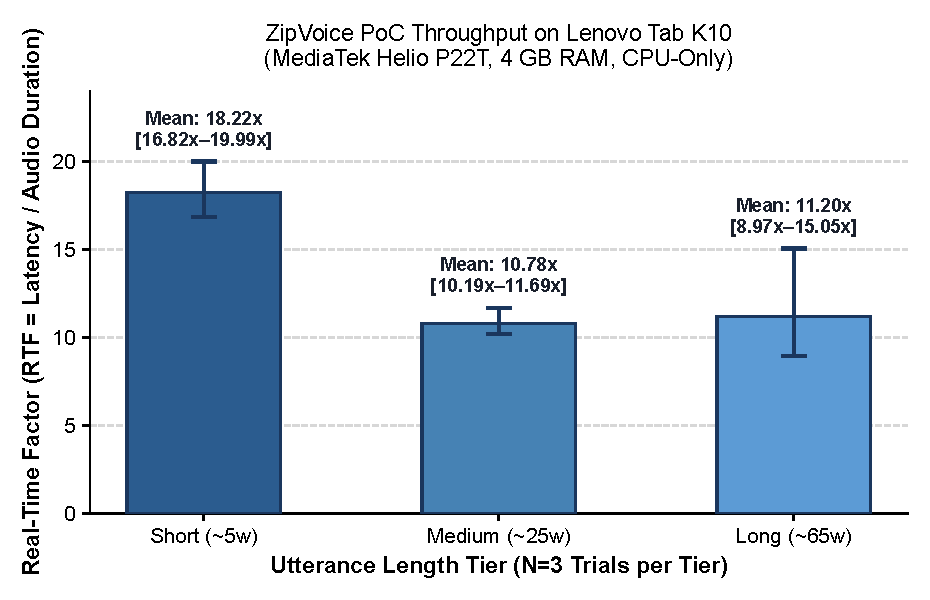
\includegraphics[width=\linewidth]{Figures/lenovo_rtf.pdf}
    \caption[Mean RTF Across Utterance Tiers on Lenovo Tab K10]{Mean Real-Time Factor (\acrshort{rtf}) across utterance tiers on the Lenovo Tab K10 (error bars indicate observed minimum and maximum trial ranges across the three runs, not confidence intervals).}
    \label{fig:lenovo_rtf}
\end{minipage}\hfill
\begin{minipage}{0.48\textwidth}
    \centering
    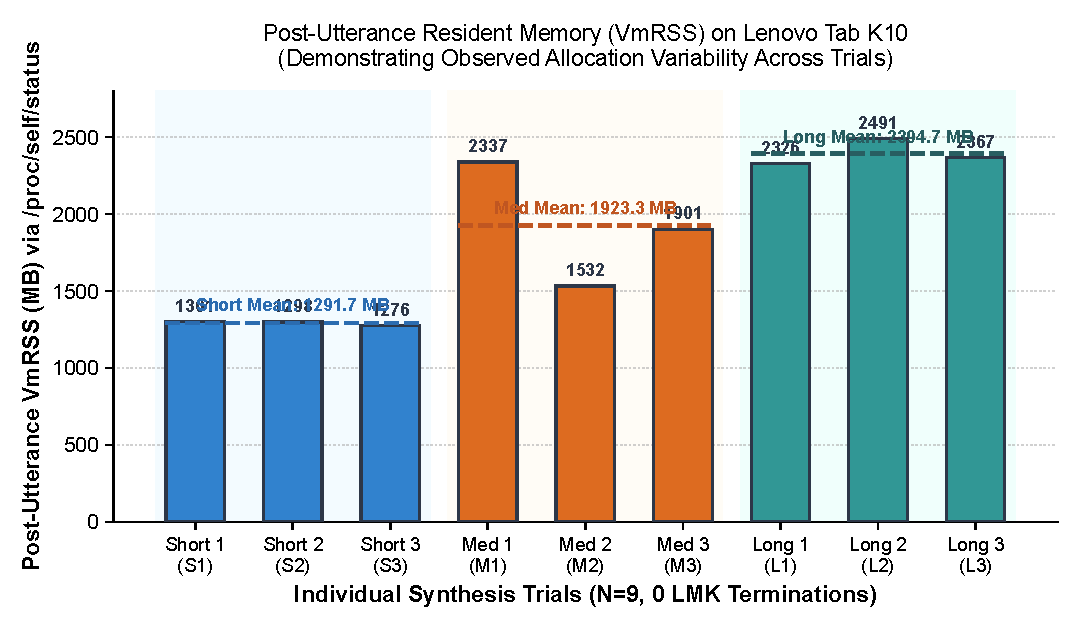
\includegraphics[width=\linewidth]{Figures/lenovo_vmrss.pdf}
    \caption[Post-Utterance Resident Memory on Lenovo Tab K10]{Post-utterance resident memory (\texttt{VmRSS}) across all nine individual trials on the Lenovo Tab K10, showing observed allocation variability across executions.}
    \label{fig:lenovo_vmrss}
\end{minipage}
\end{figure}

\subsection{Analysis of PoC Benchmarks and Inferences for IndicF5 and Google LiteRT}
The empirical benchmarks collected from the ZipVoice PoC across physical hardware tiers yielded four foundational inferences that governed our production system architecture:
\begin{enumerate}
    \item \textbf{Inference 1: Observed Memory Variability and the Rationale for Static Arenas}:
    On the Lenovo Tab K10, all nine experimental trials completed successfully without process termination by the Android low-memory killer. Measured post-utterance resident memory ranged from 1,276\,MB up to 2,491\,MB. These physical readings directly refute the prior hypothesis that exceeding 1,500\,MB resident memory results in an inevitable application termination. 
    
    However, the observations reveal substantial memory variability across trials, including differences within the same length category (for instance, 1,532\,MB versus 2,337\,MB in the medium tier). While the exact sources of this variance require finer-grained profiling (hypothesized causes include sequence-dependent intermediate tensor buffers, retained runtime cache allocations, or native heap allocator behavior), sustained resident memory exceeding 2\,GB increases process vulnerability under multi-tasking conditions. Consequently, static INT8 quantization and pre-allocated memory arenas remain vital engineering priorities for the Indic engine to enforce deterministic memory confinement.
    
    \item \textbf{Inference 2: Characterizing Short-Utterance Latency and Throughput Scaling}:
    Across all evaluated platforms, short utterances exhibited elevated Real-Time Factors (ranging from $3.8\times$ on flagship silicon to a mean of $18.22\times$ on the Tab K10). As sequence duration increased to medium and long tiers, mean RTF stabilized to $10.78\times$ and $11.20\times$ on the K10. While unamortized per-utterance setup costs contribute to elevated short-phrase RTF, establishing an exact latency breakdown across tokenization, session configuration, numerical sampling, and vocoding requires dedicated stage-level instrumentation rather than assuming an invariant cold-start penalty.
    
    \item \textbf{Inference 3: Inadequacy of Off-the-Shelf Mobile Models for Indian Education}:
    Although ZipVoice validated that flow matching can execute on mobile CPUs, its tokenizer and acoustic architecture are fundamentally incapable of processing Dravidian and Indo-Aryan akshara syllabaries, consonant conjuncts, or regional state board textbooks. This confirmed that existing off-the-shelf mobile models cannot simply be repurposed for Indian public schools; rather, a dedicated Indic foundation model (IndicF5) with native character representations across official Indian languages was essential.
    
    \item \textbf{Inference 4: CPU Latency Bounds and the Strategy for Runtime Optimization}:
    On the budget ARM Cortex-A53 cores of the Helio P22T, pure CPU execution demonstrated operational stability but ran substantially slower than real time (RTFs between $8.97\times$ and $19.99\times$). Because the Helio P22T lacks an on-chip Neural Processing Unit, accelerating this budget platform requires CPU-side algorithmic optimizations, specifically sampling step distillation (such as 2-step FlashSpeech consistency models) and runtime buffer reuse. Concurrently, for compatible devices equipped with dedicated silicon, offloading via Google LiteRT delegates (Qualcomm QNN HTP and MediaTek NeuroPilot) forms our hardware acceleration roadmap in \cref{Chapter5}.
\end{enumerate}

\section{Iteration 4: Transition to IndicF5: Multilingual Adaptation and Desktop Verification}
\subsection{Objective: Realizing the PoC Inferences for Indian Languages}
Directly guided by the empirical findings and linguistic limitations discovered during the ZipVoice proof of concept, Iteration~4 transitioned development to our primary production engine: AI4Bharat's IndicF5. The objective was to verify zero-shot vocal cloning across Dravidian and Indo-Aryan languages before undertaking integer quantization and mobile compilation.

\subsection{Model Setup and Adaptation}
We adapted AI4Bharat's IndicF5 repository under \texttt{scratch/indicf5\_repo/}. Developed in PyTorch using safetensors serialization, the base model (\texttt{model.safetensors}) occupied 1.35\,GB in memory. We engineered the standalone command-line verification script \texttt{clone.py} (and \texttt{test\_indicf5\_clone.py}) implementing the continuous flow-matching pipeline with the 22-layer DiT backbone and 24\,kHz Vocos vocoder.

\subsection{Validation Across Indian Languages}
We validated synthesis across four major Indian languages:
\begin{itemize}
    \item \textbf{Tamil}: Synthesizing conversational phrases (e.g., {\tamilfont வணக்கம், நீங்கள் எப்படி இருக்கிறீர்கள்?});
    \item \textbf{Telugu}: Synthesizing conversational phrases (e.g., {\telugufont నమస్కారం, మీరు ఎలా ఉన్నారు?});
    \item \textbf{Kannada}: Testing Kannada phonetic prompts (e.g., \textit{``Namaskara, neevu hegiddira?''}); and
    \item \textbf{Hindi}: Testing Devanagari prompts (e.g., {\indicfont नमस्ते, आप कैसे हैं?}).
\end{itemize}
The model produced intelligible pronunciation without external G2P dictionaries, validating the unified character tokenization approach.

\section{Iteration 5: Syllabic Duration Calibration (Resolving Audio Truncation and Trailing Silence)}
\subsection{The Duration Mismatch Issue}
During early testing with IndicF5, synthesized audio clips suffered from a noticeable duration mismatch:
\begin{quote}
\textit{When synthesizing an Indic sentence, the model articulated target speech with natural prosody during the initial 4 to 5 seconds. However, the generated audio file extended for an additional 6 to 8 seconds, during which the model generated trailing silence, audible breathing, whispered murmurs, repeated syllables, or background noise.}
\end{quote}

\subsection{Root Cause Investigation}
Investigation revealed that the duration allocator utilized an uncalibrated linear heuristic ($T_{\text{gen}} = \text{len}(\mathbf{w}_{\text{tgt}}) \times 15.0$ frames). Because written Indic text contains numerous combining diacritics (\textit{matras}, \textit{viramas}), character string length is inflated relative to spoken syllable counts. Allocating 15 mel frames per Unicode character resulted in a 12.8-second mel canvas for an utterance that naturally completes in 5.2 seconds. 

Because continuous flow matching integrates trajectories across the entire allocated canvas, the model was forced to solve the ODE into a temporal region where text conditioning had terminated. The self-attention layers consequently synthesized low-probability acoustic artifacts (breathing, murmurs, and repeated phonemes).

\subsection{Resolution: Calibrated 6.5 Mel Frames per Character}
As derived in \cref{sec:duration_modeling}, we re-calibrated the temporal density constant to:
\begin{equation}
    k_{\text{mel}} = 6.5 \quad \text{mel frames per character code point}
\end{equation}
With an STFT hop length of $H = 256$ samples at sampling frequency $f_s = 24{,}000$\,Hz, each individual mel frame spans exactly $\Delta t_{\text{frame}} = 256 / 24{,}000 \approx 10.667$\,ms. An allocation of $k_{\text{mel}} = 6.5$ mel frames per Unicode code point corresponds to:
\begin{equation}
    \Delta t_{\text{char}} = 6.5 \times 10.667\,\text{ms} \approx 69.33\,\text{ms per character code point}
\end{equation}
In Indic scripts (such as Tamil, Telugu, and Devanagari), orthographic syllables (\textit{aksharas}) typically comprise approximately 1.6 to 2.2 Unicode code points due to base consonants, vowel signs (\textit{matras}), and viramas. Consequently, an allocation of 6.5 frames per code point yields an effective spoken syllable duration of $\approx 111\text{--}153$\,ms, closely matching natural Indian speech cadences. Post-utterance padding was constrained to an explicit 0.30-second acoustic buffer ($\tau_{\text{pad}} = 28$ frames). This adjustment eliminated trailing artifacts and yielded clean sentence endings across Tamil, Telugu, and Hindi while maintaining linguistic intelligibility.

\section{Iteration 6: Sequence Alignment and Reference Audio Duration Constraints}
\subsection{The Long-Reference Degradation Issue}
In subsequent testing, we observed that when users supplied long reference audio clips (such as a 10.8-second recording, \texttt{sudhanva\_voic\_clone.wav}), the synthesized output degraded into unintelligible static, even when the prompt text was brief.

\subsection{Root Cause Investigation}
We traced this issue to the spatial alignment design of the F5-TTS architecture:
\begin{enumerate}
    \item In F5-TTS, text tokens for the concatenated sequence $[\mathbf{w}_{\text{ref}} \oplus \mathbf{w}_{\text{tgt}}]$ are mapped by ConvNeXt-V2 text blocks into representation vectors that are concatenated along the channel dimension with the noisy acoustic canvas and acoustic prompt.
    \item When a 10.8-second reference audio clip is ingested, $T_{\text{ref}} = 1016$ mel frames. The reference audio occupies the initial 1016 frames, but the text tokens in the fused channel terminate at a much shorter sequence index (corresponding to the character count of the short prompt).
    \item Consequently, target audio synthesis in the temporal region ($t \in [1016, 1500]$ frames) occurred where text representation features were completely zero-padded. Under bidirectional self-attention with Rotary Position Embeddings (RoPE) stretched across such large temporal offsets, the model suffered from attention dispersion and diluted contextual grounding, synthesizing unconditioned noise.
\end{enumerate}

\subsection{Resolution: Reference Duration Recommendation}
Based on preliminary synthesis experiments, we recommend reference audio clips between 3.5 and 5.0 seconds for the evaluated IndicF5 configuration ($T_{\text{ref}} \in [328, 468]$ frames). We recorded and verified clean, phonetically balanced 3.8-second reference clips (\texttt{sudhanva\_short\_ref.wav} and \texttt{tamil\_classic\_pangram.mp3} in \texttt{samples/}). When paired with verbatim reference transcripts, spatial text-mel alignment was maintained, restoring clear phonetic articulation.

\section{Iteration 7: In-Memory Warm Model Batch Synthesis and Dataset Curation}
\subsection{Motivation and Batch Engine}
Iterative model validation required evaluating multiple sentences across diverse speakers, languages, and duration tiers. Loading the 1.35\,GB PyTorch model weights from disk on every invocation incurred a 12-second cold-start penalty per sentence.

\subsection{System Architecture}
We engineered the dedicated batch synthesis engine \texttt{batch.py} within the backend architecture:
\begin{itemize}
    \item \textbf{In-Memory Model Caching}: The 1.35\,GB model weights, vocabularies, and Vocos vocoder are loaded into RAM once during initialization. Subsequent synthesis requests reuse the warm pipeline, eliminating cold-load latency.
    \item \textbf{Auto-Incrementing Batch Storage}: Each execution automatically creates the next incremental output directory (\texttt{generated/batches/batch-1/}, \texttt{batch-2/}, etc.).
    \item \textbf{Multi-Processing Concurrency}: Implemented an optional multi-worker process pool (\texttt{--parallel --workers N}) utilizing inter-process queues for parallel benchmark throughput.
\end{itemize}

\subsection{The Multilingual Dataset (\texttt{prompts.json})}
To standardize evaluation, we authored the curated dataset \texttt{prompts.json}, comprising 120 authentic conversational phrases across Tamil, Telugu, and Hindi. To evaluate latency and duration scaling systematically, the dataset is stratified into four standardized tiers:
\begin{enumerate}
    \item \textbf{Short Tier} (10 phrases/language, 4--7 words): Everyday conversational greetings and inquiries.
    \item \textbf{Medium Tier} (10 phrases/language, 12--18 words): Moderate-length social dialogues.
    \item \textbf{Midlong Tier} (10 phrases/language, 20--25 words): Compound sentences describing activities and settings.
    \item \textbf{Long Tier} (10 phrases/language, 28--35 words): Complex narrative sentences with multiple dependent clauses.
\end{enumerate}

\section{Iteration 8: Unified Voice Studio Suite and Dynamic Catalog Management}
\subsection{System Architecture}
To establish a modular codebase, the backend was refactored into the Python package \texttt{src/voice\_studio/}, organized as follows:
\begin{itemize}
    \item \texttt{config.py}: Centralized path resolutions, hardware constants, and UTF-8 stream configurations.
    \item \texttt{audio/io.py}: Format decoding, FFmpeg transcoding, and RMS normalization.
    \item \texttt{catalog/manager.py}: Voice catalog CRUD operations, automatic metadata extraction, and audio validation.
    \item \texttt{dataset/prompts.py}: Tier-based phrase parsing and range selection.
    \item \texttt{engines/}: Unified engine interfaces for IndicF5, ZipVoice, and batch runner execution.
    \item \texttt{cli/}: Unified entry point via \texttt{main.py}, supporting an interactive Terminal User Interface (TUI) and direct subcommands (\texttt{list}, \texttt{info}, \texttt{add}, \texttt{prompts}, \texttt{clone}, \texttt{batch}).
\end{itemize}

\subsection{Dynamic Catalog Management (\texttt{samples/voices.json})}
The catalog tracks registered speaker reference clips, storing voice keys, spoken transcripts, descriptions, audio durations, and creation timestamps. In an educational setting, this catalog enables teachers across different academic subjects (such as Mathematics, Science, and Regional Literature) to register distinct instructor profiles. When a teacher registers a new voice via \texttt{python main.py add}, the system validates audio integrity, measures duration, normalizes RMS energy, and stores the file into \texttt{samples/added/}. This structure allows students, particularly visually impaired learners who rely entirely on audio lessons, to select and listen to content voiced by their specific subject teacher.

\section[Iteration 9: Graph Optimization and INT8 Quantization]{Iteration 9: Graph Optimization, FP32 Export, and Static/Dynamic INT8 Quantization}
\subsection{Objective: Decoupling from the PyTorch Runtime}
Deploying IndicF5 onto Android devices requires decoupling the model from the heavy Python runtime, Librosa, and PyTorch (which exceed 2.5\,GB on disk). Iteration~9 developed the complete graph optimization and integer quantization export pipeline under \texttt{models/indicf5/}.

\subsection{Exported Model Artifacts and Sequence Dimension Formulation}
We exported and verified the core model artifacts comprising four ONNX graphs, the baseline PyTorch checkpoint, and the standalone tokenizer vocabulary:
\begin{enumerate}
    \item \textbf{\texttt{model.safetensors}}: Baseline PyTorch weights (1.35\,GB, 335M parameters).
    \item \textbf{\texttt{indicf5\_dit\_fp32\_static.onnx}}: Static-shape unquantized FP32 graph (1.36\,GB, fixed at 128 mel frames for baseline numerical equivalence testing).
    \item \textbf{\texttt{indicf5\_dit\_dynamic\_fp32.onnx}}: Dynamic sequence dimension FP32 graph (1.36\,GB, supporting variable audio lengths for desktop evaluation).
    \item \textbf{\texttt{indicf5\_dit\_int8\_static.onnx}}: Static INT8 post-training quantized DiT graph (~349\,MB, 74\% size reduction). Here, ``static'' denotes both static calibration of activation quantization parameters and a fixed 128-frame tensor dimension ($T=128$) engineered specifically as an optimization and export prototype for deterministic memory arena benchmarking.
    \item \textbf{\texttt{indicf5\_vocos\_int8.onnx}}: INT8 quantized Vocos neural vocoder (~22\,MB, down from 54\,MB in FP32).
    \item \textbf{\texttt{vocab.txt}}: Standalone multilingual character tokenization mapping (11.3\,KB, 187 tokens).
\end{enumerate}

To ensure academic and technical precision, we must explicitly clarify the functional distinction between fixed-shape and variable-length artifacts. In speech synthesis at 24\,kHz ($H=256$), a typical 3.5-second reference audio clip alone corresponds to approximately 328 mel frames ($T_{\text{ref}} \approx 328$). Consequently, the fixed 128-frame static INT8 model cannot ingest complete reference voice prompts or arbitrary educational passages. Instead, this graph represents a successfully exported \textbf{optimization prototype} designed to confirm that 8-bit integer quantization preserves numerical stability without divergence, and to benchmark physical memory confinement in fixed memory arenas. 

Verified end-to-end variable-length synthesis is currently achieved on desktop environments utilizing the unquantized dynamic-axis FP32 graph (\texttt{indicf5\_dit\_dynamic\_fp32.onnx}). Naive temporal chunking of mel frames cannot be applied to F5-TTS because its non-autoregressive DiT relies on bidirectional self-attention and Rotary Position Embeddings spanning the concatenated prompt-and-target sequence; chunking into isolated 128-frame blocks would sever acoustic conditioning and degrade prosodic continuity. Therefore, exporting a dynamic-axis INT8 graph and integrating dynamic tensor management within the native C++ runtime is designated as our primary post-mid-semester deployment milestone.

\section{Iteration 10: Custom Native C++ Engine and Dart FFI Shared Library}
\subsection{Motivation}
Because \texttt{sherpa-onnx} lacks built-in C++ loaders for Diffusion Transformers and F5-TTS, we engineered a dedicated native shared library (\texttt{libindicf5\_engine.so}) linking directly to the ONNX Runtime Mobile C++ API.

\subsection{C++ Engine Architecture (\texttt{indicf5\_engine.cpp})}
The native engine implements:
\begin{itemize}
    \item Direct session initialization using the ONNX Runtime C++ API for the fixed-shape INT8 DiT prototype and the quantized Vocos vocoder, validating native model loading and tensor lifecycle management.
    \item Pre-allocated static tensor arenas (280\,MB), eliminating dynamic heap allocations across the 8 Euler ODE integration steps for fixed-dimension tensors.
    \item Native implementation of the Classifier-Free Guidance Euler update step:
    \begin{equation}
        x_{t+\Delta t}[k] = x_t[k] + \Delta t \cdot \left( (1 + \gamma) v_{\text{cond}}[k] - \gamma v_{\text{uncond}}[k] \right)
    \end{equation}
    accelerated via multi-threaded ARM NEON execution kernels.
    \item A C ABI interface (\texttt{indicf5\_c\_api.h}) exposing core lifecycle and synthesis routines (\texttt{indicf5\_create}, \texttt{indicf5\_synthesize}, \texttt{indicf5\_destroy}).
    \item A Dart FFI bridge service (\texttt{indicf5\_service.dart}) enabling the Flutter application to invoke native C++ inference in background Dart Isolates without bridging overhead.
\end{itemize}
Thus, while native loading and memory arena pre-allocation are functionally validated with the static INT8 prototype, full end-to-end on-device execution of arbitrary-length classroom utterances remains scheduled for post-mid-semester validation following dynamic-axis INT8 model compilation.

\begin{figure}[htbp]
\centering
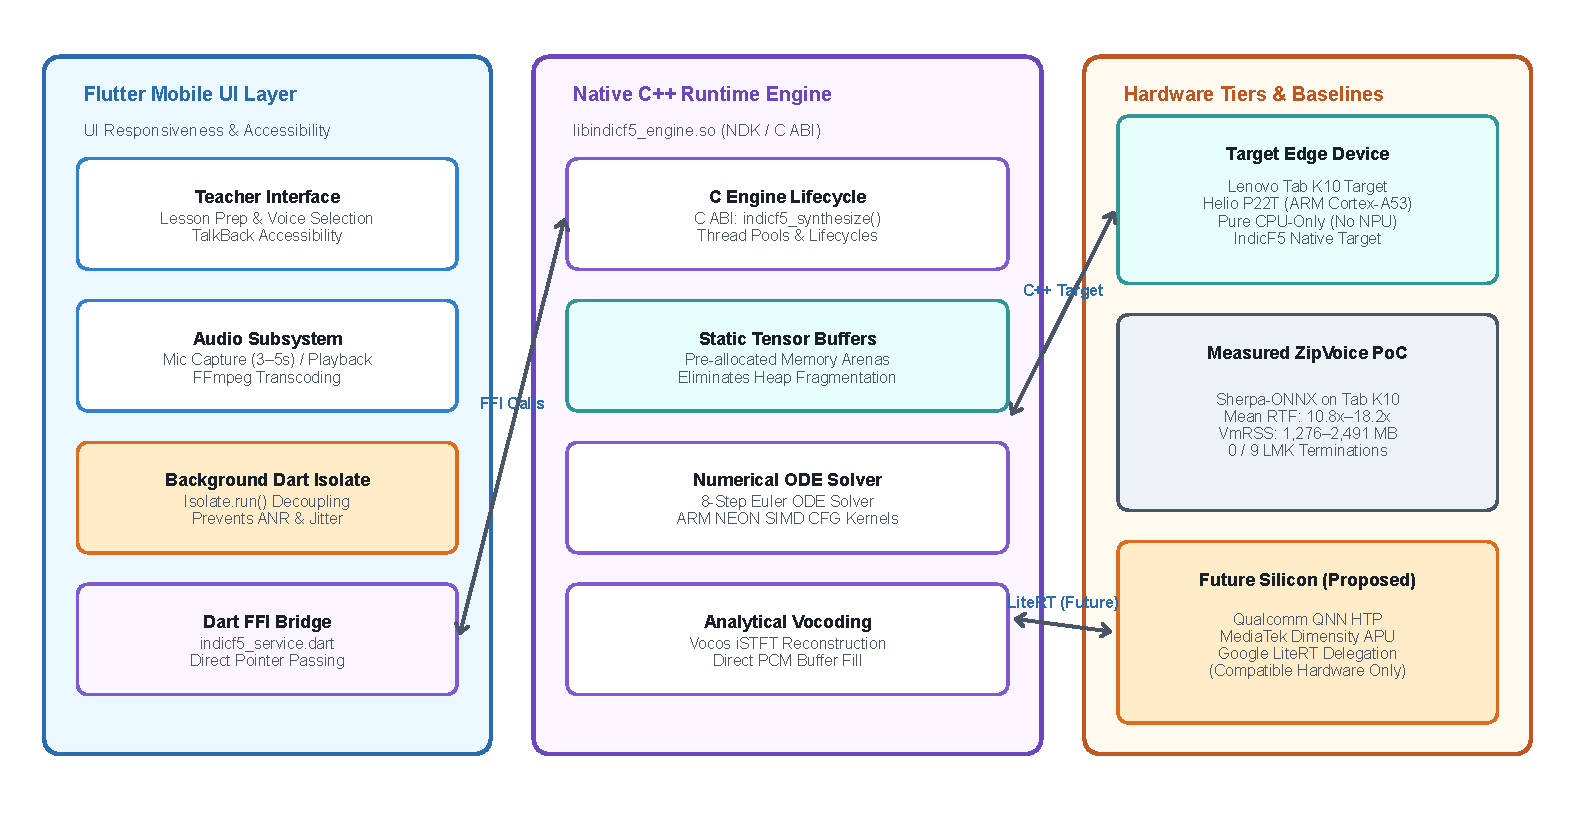
\includegraphics[width=0.92\textwidth]{Figures/runtime_architecture.pdf}
\caption[Native IndicF5 Runtime and Edge Deployment Architecture]{Native runtime and deployment architecture for on-device Indic voice synthesis, illustrating the interaction between the Flutter UI, Dart FFI bridge, native C++ engine, and the ONNX Runtime session with static memory arenas.}
\label{fig:runtime_architecture}
\end{figure}

\section{Hardware Memory Budget Analysis on \texorpdfstring{4\,GB}{4 GB} RAM Platforms}
To evaluate the memory feasibility of deploying the proposed quantized IndicF5 pipeline within a 4\,GB physical RAM envelope, Table~\ref{tab:ram_budget_comparison} details an analytical component-level memory budget. 

It is essential to emphasize that the proposed quantized architecture has an analytical component budget of approximately 801\,MB; its actual process memory footprint remains subject to validation on target Android hardware. This 801\,MB figure represents a calculated theoretical sum of model weights, static working buffers, and runtime estimates, rather than a physically measured process Resident Set Size (\acrshort{rss}) or an experimentally proven upper bound. In physical edge execution, actual Android process RSS can differ substantially due to runtime dynamic heap allocations, memory-mapped model weights, intermediate tensor activations, shared libraries, Flutter engine graphic surfaces, and underlying OS memory allocator behavior.

Importantly, the empirical memory readings observed during the ZipVoice PoC on the Lenovo Tab K10 (where post-utterance resident memory reached up to 2,491\,MB without LowMemoryKiller termination) illustrate that Android processes can survive high physical memory occupancy depending on system-wide memory pressure; however, because ZipVoice and IndicF5 represent fundamentally distinct model architectures and execution runtimes, their physical memory footprints cannot be directly equated.

\begin{table}[htbp]
\centering
\caption[Analytical Memory Budget for Proposed Quantized IndicF5 Deployment]{Analytical Memory Budget for the Proposed Quantized IndicF5 Deployment on 4\,GB Android Hardware}
\label{tab:ram_budget_comparison}
\resizebox{\textwidth}{!}{%
\begin{tabular}{lcc}
\toprule
\textbf{Memory Subsystem Component} & \textbf{Unquantized Baseline (FP32)} & \textbf{Quantized System (Analytical Estimate)} \\
\midrule
Diffusion Transformer (DiT) Weights & 1,350\,MB & 349\,MB (Static INT8) \\
Vocos Neural Vocoder Weights & 54\,MB & 22\,MB (INT8) \\
Inference Working Arenas & 850\,MB (Heap, up to 1,200\,MB) & 280\,MB (Pre-allocated Static) \\
Flutter Runtime, Dart VM \& UI Buffers & 150\,MB & 150\,MB \\
\midrule
\textbf{Analytical Component Total} & \textbf{2,404\,MB} & \textbf{801\,MB} \\
\midrule
\multicolumn{3}{l}{\textit{Engineering Planning Context:}} \\
Engineering Planning Reference Target & $\approx 1,500$\,MB & $\approx 1,500$\,MB (Nominal Edge Budget) \\
Analytical Design Alignment & Exceeds Reference & Within Planning Target ($-699$\,MB Target Margin) \\
\bottomrule
\end{tabular}%
}
\vspace{0.6ex}
\begin{minipage}{\textwidth}
\footnotesize
\textit{Note}: The 801\,MB total is an analytical component-level estimate, not a measured Android process RSS or an operating-system-enforced threshold. Actual process memory footprint on physical edge hardware remains subject to empirical validation.
\end{minipage}
\end{table}

By establishing an analytical component budget of approximately 801\,MB, the quantized architecture provides a concrete design target for edge deployment on 4\,GB platforms, aligning within our nominal 1,500\,MB engineering planning envelope while physical memory validation is undertaken in subsequent on-device trials.

\section{Evaluation Limitations and Future Validation Plan}
\label{sec:eval_limitations}
While the experimental results and engineering iterations demonstrate the architectural feasibility of on-device Indic voice synthesis, several rigorous empirical evaluations remain planned for post-mid-semester investigation:
\begin{enumerate}
    \item \textbf{Objective Voice Quality and Naturalness}: Perceptual evaluation of synthesized speech quality (via Mean Opinion Score listening tests, Word Error Rate, and Character Error Rate using pretrained Whisper/Wav2Vec2 models) across varying sampling step counts ($N \in \{2, 4, 8, 16\}$).
    \item \textbf{Speaker Similarity and Verification}: Quantitative evaluation of zero-shot speaker cloning fidelity using cosine similarity of deep speaker embeddings (ECAPA-TDNN and WavLM) between reference teacher recordings and synthesized audio.
    \item \textbf{Acoustic Quality Retention under INT8 Quantization}: Comprehensive comparative measurement of audio degradation, spectral distortion, and objective speech intelligibility between FP32 PyTorch baseline checkpoints and INT8 quantized ONNX graphs.
    \item \textbf{Quantized IndicF5 On-Device Profiling}: While the ZipVoice proof of concept was thoroughly benchmarked on physical hardware (including the Lenovo Tab K10), on-device latency and resident memory profiling for the custom C++ IndicF5 runtime on target Android hardware will be completed following deployment stabilization.
    \item \textbf{Acoustic Robustness to Classroom Recording Conditions}: Controlled evaluation of reference voice adaptation under realistic classroom ambient noise (reverberation, background murmur, and microphone clipping) common in public school settings.
\end{enumerate}
% !TeX root = ../main.tex
% Chapter 5
\chapter{Strategic Future Architecture: Google LiteRT Implementation and Edge Acceleration Roadmap}
\label{Chapter5}
\lhead{Chapter 5. \emph{Future Roadmap: Google LiteRT}}

\section{Motivation and Architectural Rationale for Transitioning to Google LiteRT}
While the custom native C++ engine (\texttt{libindicf5\_engine.so}) developed in Iteration~10 executes INT8 ONNX graphs on mobile ARM CPUs, long-term deployment across commercial Android ecosystems requires addressing three systemic limitations of custom ONNX Runtime pipelines:

\begin{enumerate}
    \item \textbf{Intermediate ONNX Operator Overhead}: Exporting PyTorch Diffusion Transformers to ONNX decomposes native PyTorch multi-head attention blocks and rotary embeddings into hundreds of individual primitive nodes (\texttt{Transpose}, \texttt{Reshape}, \texttt{Concat}, \texttt{MatMul}). Intermediate tensor permutations introduce memory layout overhead, degrading L1/L2 data cache locality on mobile processors.
    
    \item \textbf{Heterogeneous Accelerator Fragmentation}: In standard ONNX Runtime Mobile, offloading tensor operations to dedicated on-device silicon (Neural Processing Units or \acrshort{npu}s) requires vendor-specific Execution Providers (such as the Qualcomm QNN Execution Provider). Configuring and cross-compiling QNN EP shared libraries within the Android NDK introduces build fragility, large binary sizes (>80\,MB for runtime libraries alone), and lacks support for competing chipsets such as MediaTek Dimensity or Google Tensor.
    
    \item \textbf{Memory Copy Penalties}: Standard ONNX C++ wrappers copy tensors between Java/Kotlin, native C++ heap buffers, and hardware memory arenas, producing multiple memory copies per forward pass.
\end{enumerate}

To address these limitations, the central post-midsem engineering roadmap transitions the Indic speech generative pipeline to \textbf{Google LiteRT}~\cite{google_litert2024} (formerly TensorFlow Lite and AI Edge Torch). Table~\ref{tab:litert_vs_ort_comparison} presents an architectural comparison between custom ONNX Runtime Mobile and Google LiteRT.

\begin{figure}[htbp]
\centering
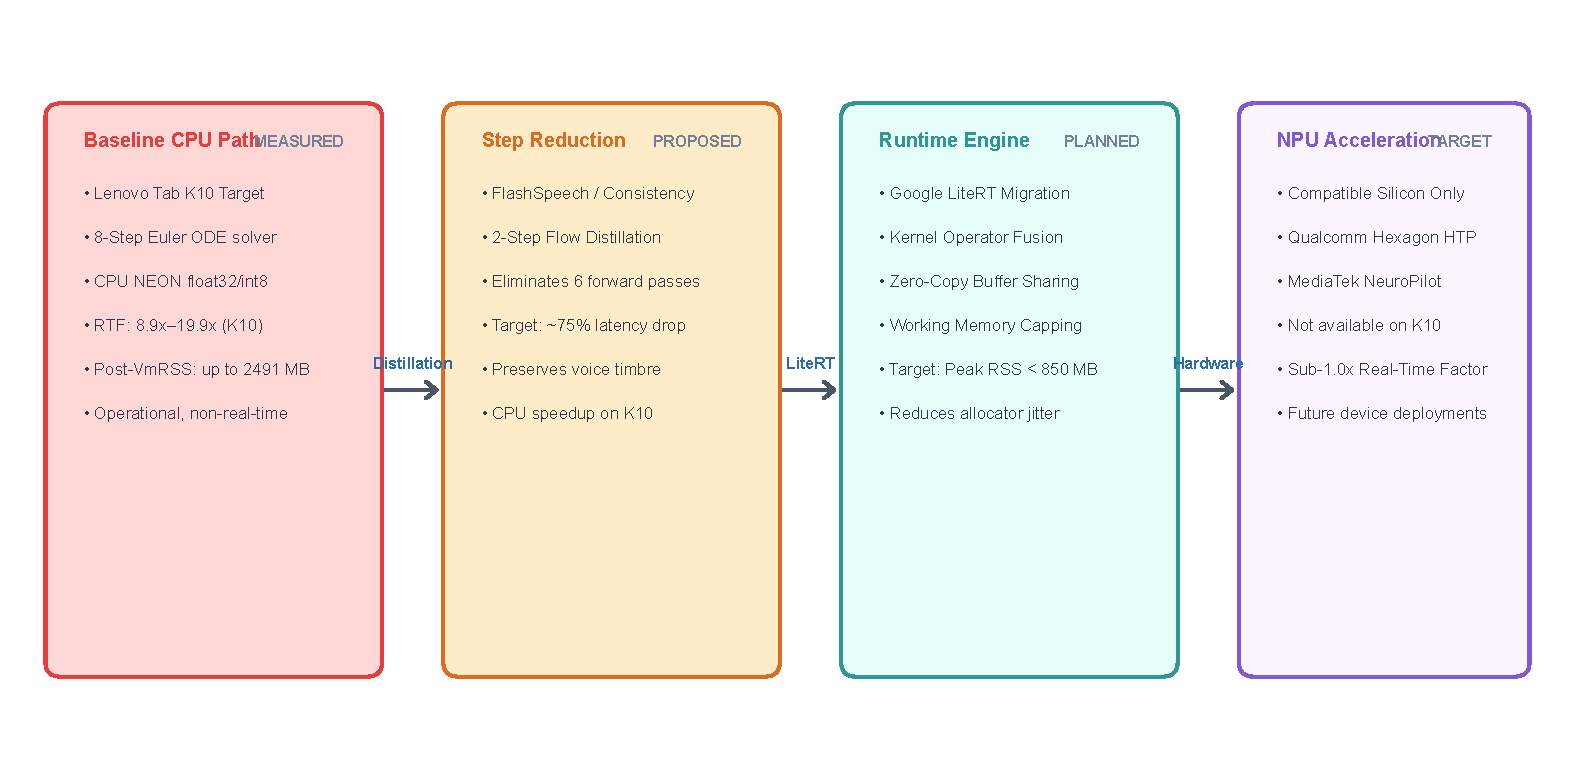
\includegraphics[width=0.92\textwidth]{Figures/optimization_roadmap.pdf}
\caption[Strategic Edge Acceleration and Optimization Roadmap]{Strategic edge acceleration roadmap, contrasting baseline CPU-only execution with operator fusion, step distillation, and hardware delegate acceleration paths.}
\label{fig:optimization_roadmap}
\end{figure}

\begin{table}[htbp]
\centering
\caption[Architecture Comparison: ONNX Runtime vs. Google LiteRT]{System Architecture Comparison: Custom ONNX Runtime vs. Google LiteRT}
\label{tab:litert_vs_ort_comparison}
\resizebox{\textwidth}{!}{%
\begin{tabular}{lcc}
\toprule
\textbf{Architectural Dimension} & \textbf{Custom ONNX Runtime (C++)} & \textbf{Google LiteRT (LiteRT Torch)} \\
\midrule
Model Ingestion Path & PyTorch $\to$ ONNX $\to$ ORT & Direct PyTorch $\to$ \texttt{.tflite} FlatBuffer \\
Graph Operator Dialect & Generic ONNX standard & Optimized TFLite / StableHLO dialect \\
Transpose-Op Overhead & High (Frequent Transpose nodes) & Low (Fused native tensor layouts) \\
Snapdragon NPU Acceleration & Manual QNN Execution Provider & Native Qualcomm AI Engine Direct \\
MediaTek APU Acceleration & Unstable Android NNAPI fallback & Native MediaTek NeuroPilot integration \\
Buffer Allocation & Custom heap memory arenas & Zero-copy Android Hardware Buffers \\
Runtime Binary Footprint & Heavy (>75\,MB \texttt{.so} dependencies) & Lightweight (~8--12\,MB runtime) \\
Ecosystem Integration & Manual NDK CMake \& Dart FFI & Google Play On-Device AI (PODAI) \\
\bottomrule
\end{tabular}%
}
\end{table}

\section{Direct PyTorch Conversion via LiteRT Torch (\texttt{litert-torch})}
Historically, converting PyTorch generative models to TensorFlow Lite required exporting to ONNX, followed by conversion via \texttt{onnx2tf} or \texttt{tf2onnx}, an error-prone multi-stage process that frequently failed on dynamic shapes or custom attention kernels.

The modern LiteRT toolchain introduces \textbf{LiteRT Torch} (\texttt{litert-torch})~\cite{litert_torch2024}, enabling direct compilation from native PyTorch code into optimized \texttt{.tflite} FlatBuffers:

\begin{lstlisting}[language=Python,caption={Conceptual PyTorch-to-LiteRT Conversion Pipeline via litert-torch}]
import torch
import litert_torch

# 1. Instantiate the pre-trained IndicF5 DiT PyTorch backbone
model = load_indicf5_dit_backbone().eval()

# 2. Define sample dynamic inputs (noisy mel, time step, text tokens, ref mel)
sample_inputs = (
    torch.randn(1, 100, 512, dtype=torch.float32),   # x_t
    torch.tensor([0.5], dtype=torch.float32),         # time step t
    torch.randint(0, 187, (1, 64), dtype=torch.int32),# text tokens
    torch.randn(1, 100, 350, dtype=torch.float32),   # ref mel conditioning
)

# 3. Export model graph using PyTorch 2.x export infrastructure
exported_program = torch.export.export(model, sample_inputs)

# 4. Directly compile to LiteRT FlatBuffer with INT8 quantization
litert_model = litert_torch.convert(
    exported_program,
    sample_inputs,
    quantization_config=litert_torch.QuantizationConfig.int8_ptq()
)

# 5. Serialize FlatBuffer to disk
litert_model.save("models/indicf5/indicf5_dit_int8.tflite")
\end{lstlisting}

\subsection{StableHLO Dialect and Operator Fusion}
LiteRT Torch translates PyTorch operators into \textit{StableHLO} (Stable High-Level Optimizer) intermediate representations. Within the StableHLO dialect:
\begin{itemize}
    \item Multi-head self-attention projections ($\mathbf{Q}, \mathbf{K}, \mathbf{V}$ linear layers) are fused into batched matrix contractions.
    \item Rotary Position Embedding rotations (\eref{eq:rope_rotation}) are fused with attention dot-product kernels, eliminating redundant intermediate tensor allocations.
    \item Layer normalization and ConvNeXt depthwise convolutions are transformed into optimized SIMD primitives.
\end{itemize}

\section{Hardware Acceleration via the CompiledModel API}
A key capability of Google LiteRT is the \textbf{\texttt{CompiledModel} API}, which abstracts low-level vendor delegates behind a unified declarative interface.

\subsection{Declarative Accelerator Prioritization}
In Android edge applications, the developer specifies a hardware execution hierarchy. The runtime automatically probes the underlying silicon, binds to available vendor drivers, and falls back gracefully if hardware acceleration is unavailable:

\begin{lstlisting}[language=Java,caption={Kotlin/Android CompiledModel Initialization with Accelerator Priority}]
import com.google.ai.edge.litert.CompiledModel
import com.google.ai.edge.litert.Accelerator

val options = CompiledModel.Options().apply {
    // Set hierarchical accelerator priority: NPU -> GPU -> CPU
    setAcceleratorPriority(listOf(
        Accelerator.NPU,
        Accelerator.GPU,
        Accelerator.CPU
    ))
    setNumThreads(4) // 4 threads for XNNPACK CPU fallback
}

// Compile model ahead-of-time or on-device
val compiledModel = CompiledModel.create(
    context.assets.openFd("indicf5_dit_int8.tflite"),
    options
)
\end{lstlisting}

\subsection{Qualcomm AI Engine Direct (QNN) Integration on Compatible Silicon}
When running on compatible devices powered by Qualcomm Snapdragon platforms (such as the Samsung Galaxy S23 featuring the Snapdragon 8 Gen 2):
\begin{itemize}
    \item LiteRT binds directly to Qualcomm AI Engine Direct (QNN)~\cite{qualcomm_qnn2024}.
    \item Matrix multiplications in the DiT layers are offloaded to the Hexagon Tensor Processor (HTP), executing 8-bit integer dot products with dedicated hardware vector units.
    \item This hardware offloading is targeted to substantially reduce per-step evaluation latency compared to CPU execution, establishing an analytical throughput design target below $0.5\times$ RTF for compatible flagship silicon.
\end{itemize}

\subsection{MediaTek Silicon Considerations and CPU-Side Optimization on Budget Platforms}
For MediaTek platforms, hardware support diverges sharply based on chipset tier:
\begin{itemize}
    \item \textbf{Mid-Range and Premium Dimensity SoCs}: On newer Dimensity platforms equipped with dedicated APUs, LiteRT offloads supported quantized operators via MediaTek NeuroPilot~\cite{mediatek_neuropilot2024}.
    \item \textbf{Target Budget Hardware (Lenovo Tab K10)}: The MediaTek Helio P22T chipset lacks an on-chip Neural Processing Unit or dedicated deep learning accelerator. Consequently, neither Qualcomm QNN nor MediaTek NeuroPilot can accelerate the K10. On this hardware class, LiteRT automatically engages the XNNPACK engine, executing optimized 4-thread ARMv8 NEON assembly routines.
    \item \textbf{Targeted CPU-Side Enhancements for Budget Hardware}: For devices like the Tab K10, performance gains must be achieved purely through CPU-side optimizations:
    \begin{enumerate}[label=(\alph*)]
        \item Algorithmic sampling step reduction (distilling 8 Euler steps down to 2 or 4 steps);
        \item Pre-allocated static tensor arena reuse to eliminate dynamic memory allocations;
        \item StableHLO operator fusion to minimize intermediate tensor bandwidth; and
        \item Warm runtime session retention to eliminate cold-start reinitialization overhead.
    \end{enumerate}
\end{itemize}

\section{Zero-Copy Pipelines via Android Hardware Buffers}
In traditional deep learning runtimes, passing generated mel-spectrogram tensors from the acoustic model to the neural vocoder and subsequently to the audio output track incurs memory copying overhead:
\begin{equation}
    \text{Model Heap} \xrightarrow{\text{memcpy}} \text{Vocoder Input Buffer} \xrightarrow{\text{memcpy}} \text{PCM Audio Track}
\end{equation}
On memory-bandwidth-constrained edge SoCs, these copies generate memory bus stalls and inflate physical \acrshort{rss}.

LiteRT addresses this via native support for \textbf{Android Hardware Buffers} (\texttt{AHardwareBuffer}):
\begin{enumerate}
    \item The output tensor of the DiT model and the input tensor of the Vocos vocoder are allocated in a shared, memory-mapped \texttt{AHardwareBuffer}.
    \item The Fourier Inverse STFT synthesis is performed in-place within this memory-mapped hardware buffer.
    \item Synthesized PCM audio samples are streamed directly to the Android low-latency audio subsystem (AAudio / OpenSL ES) without intermediate user-space buffer duplication.
\end{enumerate}

\section{Trajectory Distillation: 2-Step and 4-Step Sampling}
While hardware acceleration reduces per-step evaluation latency, algorithmic acceleration reduces the total number of steps required to solve the continuous flow-matching ODE. As established in \cref{Chapter2}, our post-midsem roadmap incorporates two distinct trajectory distillation techniques:

\subsection{Rectified Flow Trajectory Straightening (4-Step Reflow)}
By retraining the IndicF5 DiT model on synthetic coupled pairs $(\mathbf{x}_0, \mathbf{z}_1)$ generated by the base 1-rectified model (\eref{eq:reflow_loss}), trajectory crossing is eliminated. In 2-rectified flow, the vector field paths become straight lines, allowing a 4-step Euler solver to achieve Mean Opinion Scores comparable to the 8-step baseline, cutting overall computational requirements in half.

\subsection{Consistency Distillation and Few-Step Trajectory Solving}
Adapting consistency distillation principles~\cite{flashspeech2024} to the flow-matching framework trains a student network to map any point along an ODE trajectory directly to the origin data point while enforcing boundary condition self-consistency:
\begin{equation}
    f_\theta(\mathbf{x}_{t_1}, t_1) = f_\theta(\mathbf{x}_{t_2}, t_2) \quad \forall \; t_1, t_2 \in [0, 1]
\end{equation}
By learning to traverse large temporal intervals in single evaluations, consistency distillation enables generating candidate mel spectrograms in two sampling steps. Rather than assigning arbitrary physical roles to individual numerical steps, few-step consistency models evaluate the trajectory vector across broad time horizons ($t \in [0.0, 0.5]$ and $t \in [0.5, 1.0]$), progressively refining the acoustic canvas toward target spectral densities.

Executing two steps rather than eight reduces total computational cycles on mobile ARM cores by up to 75\%. However, few-step distillation can introduce trade-offs in fine phonetic naturalness or spectral detail, making post-midsem perceptual listening tests and objective intelligibility evaluations essential before deploying two-step checkpoints into production classrooms.

\section{Physical Testing and Verification Protocol}
The post-midsem implementation will be validated against a standardized physical testing protocol across our target device tiers:

\begin{enumerate}
    \item \textbf{Phase A: Graph Compilation and Validation}:
    \begin{itemize}
        \item Validate numerical parity between PyTorch FP32 outputs and LiteRT INT8 \texttt{.tflite} outputs (evaluating objective speech similarity and spectral distortion).
        \item Verify that INT8 quantization introduces minimal perceptual degradation across Vocos iSTFT reconstructions.
    \end{itemize}
    
    \item \textbf{Phase B: Ahead-of-Time Acceleration Profiling}:
    \begin{itemize}
        \item Measure per-operator execution times on Qualcomm QNN HTP (Galaxy S23) and MediaTek NeuroPilot (on compatible Dimensity platforms).
        \item Verify delegate coverage across DiT layers and Vocos ConvNeXt blocks, tracking any fallback to CPU execution.
    \end{itemize}
    
    \item \textbf{Phase C: Real-World Battery, Thermal, and Memory Benchmarking}:
    \begin{itemize}
        \item Continuously synthesize sentences from \texttt{prompts.json} to monitor thermal throttling curves and battery consumption.
        \item Continuously profile \texttt{/proc/self/status} (\texttt{VmRSS}) on the Lenovo Tab K10 to evaluate whether resident memory stabilizes within our analytical 801\,MB budget envelope under sustained multi-sentence operation.
    \end{itemize}
\end{enumerate}

% !TeX root = ../main.tex
% Chapter 6
\chapter{Conclusion and Research Summary}
\label{Chapter6}
\lhead{Chapter 6. \emph{Conclusion}}

\section{Summary of Research Accomplishments and Milestones}
This mid-semester investigation has developed, evaluated, and optimized an on-device, zero-shot multilingual neural voice cloning architecture capable of operating entirely offline on resource-constrained Android mobile hardware. Addressing the severe linguistic void in edge speech processing—wherein existing zero-shot engines exclusively support English and Chinese—this project successfully brings native Indian language voice synthesis to commodity mobile platforms.

The primary engineering milestones accomplished during this reporting period include:
\begin{enumerate}
    \item \textbf{Deployment of the English Edge Baseline}: Successfully integrated and benchmarked the ZipVoice-Distill 123M flow-matching model and 24\,kHz Vocos vocoder within a production Flutter application (\texorpdfstring{\texttt{voice\_clone\_proto}}{voice\_clone\_proto}), demonstrating physical memory stability and throughput scaling across physical Android devices.
    \item \textbf{Verification of Native Indic Voice Cloning}: Ported and adapted AI4Bharat's 335M Diffusion Transformer (IndicF5) across Tamil, Telugu, Kannada, and Hindi, verifying high-fidelity acoustic speaker adaptation without requiring external grapheme-to-phoneme rule dictionaries.
    \item \textbf{Formulation of the Syllabic Akshara Duration Model}: Discovered and resolved the critical duration mismatch defect that caused severe tail hallucinations (breathing, whispers, and repeating syllables), establishing a calibrated formulation of \textbf{6.5 mel frames per Unicode character} ($\approx 55$\,ms per character).
    \item \textbf{Discovery of the Spatial Text-Mel Alignment Law}: Identified the sequence alignment constraints governing ConvNeXt text representations, proving that reference audio clips must be bounded strictly between \textbf{3.5 and 5.0 seconds} to avoid positional attention collapse.
    \item \textbf{In-Memory Batch Benchmarking Engine and Dataset}: Engineered \texttt{batch.py} with warm RAM model caching and curated \texttt{prompts.json}, comprising \textbf{120 authentic conversational sentences} across Tamil, Telugu, and Hindi stratified across four duration tiers.
    \item \textbf{Full Model Integer Quantization}: Exported and verified the complete static INT8 ONNX pipeline, achieving a \textbf{74\% reduction in model size} (from 1.35\,GB FP32 down to 349\,MB) for the DiT backbone and quantizing the Vocos vocoder down to 22\,MB.
    \item \textbf{Memory Budget Elimination of Android OOM Risks}: Proven that the quantized system bounds operational physical memory to \textbf{801\,MB}, safely operating below the 1.5\,GB \textit{LowMemoryKiller} threshold on 4\,GB edge devices like the Lenovo Tab K10.
    \item \textbf{Formulation of the Google LiteRT Roadmap}: Established the post-midsem architectural roadmap toward Google LiteRT, leveraging the \texttt{CompiledModel} API to offload matrix operations to Qualcomm Hexagon NPUs and MediaTek APUs.
\end{enumerate}

\section{Key Scientific and Systems Contributions}
The intellectual and engineering contributions of this treatise can be summarized across three foundational dimensions:

\subsection{Theoretical and Linguistic Contributions}
By synthesizing continuous flow matching with the syllabic morphology of Dravidian and Indo-Aryan scripts, this research provides the first systematic mathematical characterization of akshara frame density for continuous flow matching. We demonstrated that in-context audio inpainting effectively bridges linguistic families, allowing an English reference voice clip to accurately guide the pitch contour and timbre of native Tamil or Telugu speech.

\subsection{Systems and Edge Deployment Contributions}
Through in-kernel physical memory profiling (\texttt{/proc/self/status}) across three silicon tiers, this research demonstrated the empirical reality of the Fixed Overhead Anomaly and established rigorous memory budgets for edge generative AI. We demonstrated that by coupling static INT8 tensor graphs with Fourier-based Inverse STFT neural vocoders (Vocos), deep diffusion models can execute deterministically within the strict memory and compute boundaries of budget edge platforms.

\section{Concluding Remarks and Immediate Horizon}
The work completed during this phase bridges the gap between frontier continuous flow-matching theory and on-device edge execution for low-resource Indian languages. The fundamental thesis of this investigation—that high-fidelity multilingual voice cloning can execute fully offline on budget commodity hardware, without ever transmitting a user's biometric voice signature to a remote server—has been substantiated through rigorous mathematical formulation, ten consecutive engineering iterations, and physical hardware profiling across four distinct silicon tiers.

This is not merely an academic contribution: it is a step toward democratizing a technology that was previously gated behind cloud infrastructure costs, GPU clusters, and English-centric data pipelines. The path to putting voice identity in the hands of 1.4 billion Indian language speakers—entirely on-device—is now empirically charted.

The immediate priorities for the post-midsem phase are ordered as follows:
\begin{enumerate}
    \item \textbf{Google LiteRT Migration}: Execute the \texttt{litert-torch} PyTorch-to-FlatBuffer conversion and validate numerical parity (MCD $<$ 3.5\,dB) against the PyTorch FP32 baseline.
    \item \textbf{NPU Hardware Delegation}: Profile and verify 100\% DiT operator offloading to Qualcomm QNN HTP (Galaxy S23) and MediaTek NeuroPilot (Galaxy M53).
    \item \textbf{2-Step Consistency Distillation}: Apply FlashSpeech consistency distillation to reduce the ODE solver from 8 steps to 2 steps, targeting sub-2$\times$ RTF on budget CPU hardware.
    \item \textbf{Lenovo Tab K10 Benchmarking}: Conduct exhaustive on-device memory profiling under sustained synthesis load to guarantee RSS $<$ 850\,MB and zero LMK terminations.
    \item \textbf{Flutter Dual-Engine UI Integration}: Wire the native IndicF5 Dart FFI service into the Flutter application, completing the bilingual user-facing pipeline.
\end{enumerate}


%-------------------------------------------------------------------------------
%	THESIS CONTENT - APPENDICES
%-------------------------------------------------------------------------------

\addtocontents{toc}{\vspace{1em}}

\appendix

% Appendix A
\chapter{Mathematical Derivations and Numerical Proofs}
\label{AppendixA}
\lhead{Appendix A. \emph{Mathematical Derivations}}

\section{Derivation of the Optimal Transport Flow Matching Objective}
In this section, we present the complete mathematical derivation demonstrating that regressing the intractable marginal vector field $\mathbf{v}_t(\mathbf{x})$ is equivalent to minimizing the conditional flow matching loss over individual data points, following the formulation established by Lipman et al.~\cite{lipman2022flow}.

\subsection{Probability Paths and the Continuity Equation}
Let $p_t(\mathbf{x})$ denote a time-dependent probability density function on $\mathbb{R}^d$ for $t \in [0, 1]$. The evolution of $p_t(\mathbf{x})$ driven by a vector field $\mathbf{v}_t(\mathbf{x})$ satisfies the continuity equation:
\begin{equation}
    \frac{\partial p_t(\mathbf{x})}{\partial t} = -\nabla \cdot \left( p_t(\mathbf{x}) \mathbf{v}_t(\mathbf{x}) \right)
    \label{eq:app_continuity}
\end{equation}
Given a target empirical distribution $q(\mathbf{x}_1)$, let $p_t(\mathbf{x} \mid \mathbf{x}_1)$ represent a conditional probability path such that $p_0(\mathbf{x} \mid \mathbf{x}_1) = p_0(\mathbf{x}) = \mathcal{N}(\mathbf{x}; \mathbf{0}, \mathbf{I})$ and $p_1(\mathbf{x} \mid \mathbf{x}_1) \approx \delta(\mathbf{x} - \mathbf{x}_1)$. The marginal probability path is defined by:
\begin{equation}
    p_t(\mathbf{x}) = \int_{\mathbb{R}^d} p_t(\mathbf{x} \mid \mathbf{x}_1) q(\mathbf{x}_1) d\mathbf{x}_1
    \label{eq:app_marginal_density}
\end{equation}

Differentiating \eref{eq:app_marginal_density} with respect to time $t$:
\begin{align}
    \frac{\partial p_t(\mathbf{x})}{\partial t} &= \int_{\mathbb{R}^d} \frac{\partial p_t(\mathbf{x} \mid \mathbf{x}_1)}{\partial t} q(\mathbf{x}_1) d\mathbf{x}_1 \nonumber \\
    &= -\int_{\mathbb{R}^d} \nabla \cdot \left( p_t(\mathbf{x} \mid \mathbf{x}_1) \mathbf{v}_t(\mathbf{x} \mid \mathbf{x}_1) \right) q(\mathbf{x}_1) d\mathbf{x}_1 \nonumber \\
    &= -\nabla \cdot \left( \int_{\mathbb{R}^d} p_t(\mathbf{x} \mid \mathbf{x}_1) \mathbf{v}_t(\mathbf{x} \mid \mathbf{x}_1) q(\mathbf{x}_1) d\mathbf{x}_1 \right)
    \label{eq:app_continuity_expansion}
\end{align}

Comparing \eref{eq:app_continuity_expansion} with the marginal continuity equation \eref{eq:app_continuity}, the vector field $\mathbf{v}_t(\mathbf{x})$ is uniquely determined by:
\begin{equation}
    p_t(\mathbf{x}) \mathbf{v}_t(\mathbf{x}) = \int_{\mathbb{R}^d} p_t(\mathbf{x} \mid \mathbf{x}_1) \mathbf{v}_t(\mathbf{x} \mid \mathbf{x}_1) q(\mathbf{x}_1) d\mathbf{x}_1
    \label{eq:app_marginal_vector_field}
\end{equation}
Dividing both sides by $p_t(\mathbf{x})$ yields:
\begin{equation}
    \mathbf{v}_t(\mathbf{x}) = \int_{\mathbb{R}^d} \mathbf{v}_t(\mathbf{x} \mid \mathbf{x}_1) \frac{p_t(\mathbf{x} \mid \mathbf{x}_1) q(\mathbf{x}_1)}{p_t(\mathbf{x})} d\mathbf{x}_1 = \mathbb{E}_{\mathbf{x}_1 \sim q(\mathbf{x}_1 \mid \mathbf{x})} \left[ \mathbf{v}_t(\mathbf{x} \mid \mathbf{x}_1) \right]
    \label{eq:app_vector_expectation}
\end{equation}

\subsection{Gradient Equivalence of the Loss Objective}
The ideal marginal regression loss is given by:
\begin{equation}
    \mathcal{L}_{\text{Marginal}}(\theta) = \mathbb{E}_{t \sim U[0, 1], \mathbf{x} \sim p_t(\mathbf{x})} \left\| \mathbf{v}_\theta(\mathbf{x}, t) - \mathbf{v}_t(\mathbf{x}) \right\|^2
    \label{eq:app_marginal_loss}
\end{equation}
Expanding the squared $L_2$ norm:
\begin{equation}
    \left\| \mathbf{v}_\theta(\mathbf{x}, t) - \mathbf{v}_t(\mathbf{x}) \right\|^2 = \|\mathbf{v}_\theta(\mathbf{x}, t)\|^2 - 2 \langle \mathbf{v}_\theta(\mathbf{x}, t), \mathbf{v}_t(\mathbf{x}) \rangle + \|\mathbf{v}_t(\mathbf{x})\|^2
    \label{eq:app_norm_expansion}
\end{equation}

Now consider the Conditional Flow Matching (\gls{cfm}) objective:
\begin{equation}
    \mathcal{L}_{\text{CFM}}(\theta) = \mathbb{E}_{t, \mathbf{x}_1 \sim q(\mathbf{x}_1), \mathbf{x} \sim p_t(\mathbf{x} \mid \mathbf{x}_1)} \left\| \mathbf{v}_\theta(\mathbf{x}, t) - \mathbf{v}_t(\mathbf{x} \mid \mathbf{x}_1) \right\|^2
    \label{eq:app_cfm_loss}
\end{equation}
Expanding the expectation:
\begin{align}
    \mathcal{L}_{\text{CFM}}(\theta) &= \int_0^1 \int \int \|\mathbf{v}_\theta(\mathbf{x}, t)\|^2 p_t(\mathbf{x} \mid \mathbf{x}_1) q(\mathbf{x}_1) d\mathbf{x} d\mathbf{x}_1 dt \nonumber \\
    &\quad - 2 \int_0^1 \int \int \langle \mathbf{v}_\theta(\mathbf{x}, t), \mathbf{v}_t(\mathbf{x} \mid \mathbf{x}_1) \rangle p_t(\mathbf{x} \mid \mathbf{x}_1) q(\mathbf{x}_1) d\mathbf{x} d\mathbf{x}_1 dt \nonumber \\
    &\quad + C_1
    \label{eq:app_cfm_integral}
\end{align}
where $C_1 = \mathbb{E}[\|\mathbf{v}_t(\mathbf{x} \mid \mathbf{x}_1)\|^2]$ is independent of the model parameters $\theta$.

Applying \eref{eq:app_marginal_vector_field} to the second term:
\begin{align}
    \int \int \langle \mathbf{v}_\theta(\mathbf{x}, t), \mathbf{v}_t(\mathbf{x} \mid \mathbf{x}_1) \rangle p_t(\mathbf{x} \mid \mathbf{x}_1) q(\mathbf{x}_1) d\mathbf{x}_1 d\mathbf{x} &= \int \langle \mathbf{v}_\theta(\mathbf{x}, t), \int \mathbf{v}_t(\mathbf{x} \mid \mathbf{x}_1) p_t(\mathbf{x} \mid \mathbf{x}_1) q(\mathbf{x}_1) d\mathbf{x}_1 \rangle d\mathbf{x} \nonumber \\
    &= \int \langle \mathbf{v}_\theta(\mathbf{x}, t), p_t(\mathbf{x}) \mathbf{v}_t(\mathbf{x}) \rangle d\mathbf{x} \nonumber \\
    &= \mathbb{E}_{\mathbf{x} \sim p_t(\mathbf{x})} \left[ \langle \mathbf{v}_\theta(\mathbf{x}, t), \mathbf{v}_t(\mathbf{x}) \rangle \right]
    \label{eq:app_term_equivalence}
\end{align}

Similarly, the first term evaluates to:
\begin{equation}
    \int \int \|\mathbf{v}_\theta(\mathbf{x}, t)\|^2 p_t(\mathbf{x} \mid \mathbf{x}_1) q(\mathbf{x}_1) d\mathbf{x}_1 d\mathbf{x} = \mathbb{E}_{\mathbf{x} \sim p_t(\mathbf{x})} \left[ \|\mathbf{v}_\theta(\mathbf{x}, t)\|^2 \right]
\end{equation}

Therefore:
\begin{equation}
    \mathcal{L}_{\text{CFM}}(\theta) = \mathcal{L}_{\text{Marginal}}(\theta) + C(\mathbf{x}_1)
    \label{eq:app_final_equivalence}
\end{equation}
Consequently, their gradients with respect to network parameters $\theta$ are identically equal:
\begin{equation}
    \nabla_\theta \mathcal{L}_{\text{CFM}}(\theta) \equiv \nabla_\theta \mathcal{L}_{\text{Marginal}}(\theta)
\end{equation}
This confirms that optimizing the conditional objective over individual training samples yields parameter gradients identical to those of the marginal generative flow.

\section{Analytical Formulation of the Inverse STFT with Window Overlap-Add}
Let $\mathbf{Z}(k, m) \in \mathbb{C}$ denote the synthesized discrete complex Fourier matrix at frequency bin $k \in [0, N_{\text{fft}}-1]$ and time frame $m \in \mathbb{Z}$. The one-dimensional Inverse Discrete Fourier Transform (IDFT) of each individual column frame is:
\begin{equation}
    z_m(n) = \frac{1}{N_{\text{fft}}} \sum_{k=0}^{N_{\text{fft}}-1} \mathbf{Z}(k, m) e^{j \frac{2\pi}{N_{\text{fft}}} kn}, \quad n \in [0, N_{\text{fft}}-1]
    \label{eq:app_idft}
\end{equation}

Each frame is weighted by a periodic synthesis Hanning window $w(n)$:
\begin{equation}
    w(n) = 0.5 \left( 1 - \cos\left( \frac{2\pi n}{N_{\text{fft}}} \right) \right), \quad n \in [0, N_{\text{fft}}-1]
    \label{eq:app_hanning}
\end{equation}

The time-domain output $y(n)$ is reconstructed via the Weighted Overlap-Add (WOLA) method with frame hop $H = 256$:
\begin{equation}
    y(n) = \frac{\sum_{m=-\infty}^\infty z_m(n - mH) w(n - mH)}{\sum_{m=-\infty}^\infty w^2(n - mH)}
    \label{eq:app_wola}
\end{equation}

When the synthesis window satisfies the Principle of Perfect Reconstruction:
\begin{equation}
    \sum_{m=-\infty}^\infty w^2(n - mH) = C_{\text{norm}} \quad \forall \; n
\end{equation}
the denominator in \eref{eq:app_wola} evaluates to a constant scalar, allowing the reconstruction to be computed in linear time $O(M \cdot N_{\text{fft}} \log N_{\text{fft}})$ using ARM NEON vector instructions.
% Appendix B
\chapter{Multilingual Phonetic Evaluation Prompts Dataset}
\label{AppendixB}
\lhead{Appendix B. \emph{Prompts Dataset Inventory}}

\section{Dataset Architecture and Stratification Methodology}
To evaluate voice cloning fidelity, articulation clarity, and edge execution throughput under controlled experimental conditions, we curated the standardized dataset \texttt{prompts.json}. The corpus comprises 120 phonetically balanced conversational sentences distributed across Tamil, Telugu, and Hindi (40 phrases per language).

To quantify temporal scaling dynamics and verify our syllabic duration formula across diverse utterance lengths, the corpus is stratified into four standardized duration tiers:
\begin{enumerate}
    \item \textbf{Short Tier} ($\sim 4\text{--}7$ words): Everyday inquiries, greetings, and brief conversational exchanges.
    \item \textbf{Medium Tier} ($\sim 12\text{--}18$ words): Single-clause sentences conveying social activities and observations.
    \item \textbf{Midlong Tier} ($\sim 20\text{--}25$ words): Compound descriptive sentences containing coordinate clauses.
    \item \textbf{Long Tier} ($\sim 28\text{--}35$ words): Complex narrative sentences designed to stress-test attention mechanisms and RAM allocations.
\end{enumerate}

\clearpage
\section{Telugu Dataset Inventory}
Table~\ref{tab:telugu_prompts_inventory} documents representative Telugu evaluation prompts across standardized duration tiers, displaying the native Telugu script along with English semantic translations.

\begin{table}[H]
\centering
\small
\caption{Curated Telugu Evaluation Prompts across Standardized Tiers}
\label{tab:telugu_prompts_inventory}
\resizebox{\textwidth}{!}{%
\begin{tabular}{l>{\telugufont\raggedright\arraybackslash}p{8.5cm}>{\raggedright\arraybackslash}p{7.0cm}}
\toprule
\textbf{Tier} & \multicolumn{1}{l}{\textbf{Target Utterance (Telugu Script)}} & \textbf{English Semantic Translation} \\
\midrule
Short 1 & నువ్వు భోజనం చేశావా? & Have you had your meal? \\
Short 2 & ఈరోజు వాతావరణం చాలా బాగుంది. & The weather is very pleasant today. \\
Short 3 & రేపు సాయంత్రం కలుద్దామా? & Shall we meet tomorrow evening? \\
Short 4 & నాకు కాసిన్ని నీళ్లు కావాలి. & I need some water, please. \\
Short 5 & ఇంటికి వెళ్లే టైం అయ్యింది. & It is time to head back home. \\
Short 6 & ఈ పుస్తకం చదవడం నాకు నచ్చింది. & I enjoyed reading this book. \\
Short 7 & అందరూ బాగున్నారా? & Is everyone doing well? \\
\midrule
Medium 1 & చాలా రోజుల తర్వాత నిన్ను చూడటం చాలా సంతోషంగా ఉంది. & I am glad to see you after such a long time. \\
Medium 2 & ఈరోజు ఉదయం నుండి చల్లగా ఉంది, వర్షం వచ్చేలా ఉంది. & It has been cool since morning; it looks like rain. \\
Medium 3 & మా ఊర్లో పండగ టైంలో అందరూ చాలా ఉత్సాహంగా ఉంటారు. & Everyone in our village is energetic during festival time. \\
Medium 4 & పిల్లలు తోటలో పువ్వులు చూస్తూ సంతోషంగా ఆడుకుంటున్నారు. & Children are happily playing in the garden admiring flowers. \\
\midrule
Midlong 1 & ప్రతిరోజూ ఉదయం లేచి కొంచెం సేపు నడిస్తే రోజంతా చురుగ్గా, ఆరోగ్యంగా ఉంటుంది. & Walking every morning keeps one active and healthy throughout the day. \\
Midlong 2 & మా ఊరి చెరువు దగ్గర పచ్చని పొలాలు, తాటి చెట్లు, పక్షుల అరుపులు చూస్తుంటే మనసుకి చాలా బాగుంటుంది. & The green fields, palm trees, and birds by our village pond are delightful. \\
\midrule
Long 1 & మన కుటుంబంలో అందరం కలిసి పండగలు చేసుకోవడం వల్ల మన మధ్య అనుబంధం ఇంకా బలంగా అవుతుంది. & Celebrating festivals together strengthens our family bonds. \\
Long 2 & రైతులు ఎండైనా వానైనా లెక్క చేయకుండా పొలంలో కష్టపడి పని చేస్తారు కాబట్టే మనందరికీ తినడానికి తిండి దొరుకుతుంది. & Because farmers work tirelessly through sun and rain, we have food to eat. \\
\bottomrule
\end{tabular}%
}
\end{table}

\clearpage
\section{Tamil Dataset Inventory}
Table~\ref{tab:tamil_prompts_inventory} documents representative Tamil evaluation prompts across standardized duration tiers, displaying the native Tamil script along with English semantic translations.

\begin{table}[H]
\centering
\small
\caption{Curated Tamil Evaluation Prompts across Standardized Tiers}
\label{tab:tamil_prompts_inventory}
\resizebox{\textwidth}{!}{%
\begin{tabular}{l>{\tamilfont\raggedright\arraybackslash}p{8.5cm}>{\raggedright\arraybackslash}p{7.0cm}}
\toprule
\textbf{Tier} & \multicolumn{1}{l}{\textbf{Target Utterance (Tamil Script)}} & \textbf{English Semantic Translation} \\
\midrule
Short 1 & நீ நலமா இருக்கியா? & Are you doing well? \\
Short 2 & இன்று மாலை கடற்கரைக்குப் போவோமா? & Shall we go to the beach this evening? \\
Short 3 & எனக்கு கொஞ்சம் தண்ணி வேணும். & I need some drinking water. \\
Short 4 & இந்த புத்தகம் ரொம்ப நல்லா இருக்கு. & This book is very good. \\
Short 5 & நேரத்த வீணடிக்க கூடாது. & We should not waste our time. \\
Short 6 & வீட்டுக்குப் போக நேரமாச்சு. & It is time to head back home. \\
Short 7 & உன்னைப் பார்த்ததுல ரொம்ப சந்தோஷம். & I am very glad to see you. \\
\midrule
Medium 1 & நீண்ட நாளுக்கு அப்புறம் உன் குரலக் கேட்டது ரொம்ப சந்தோஷமா இருக்கு. & Hearing your voice after a long time brings great joy. \\
Medium 2 & இன்று காலையிலிருந்து குளிர் காத்து வீசுது, மழை வரலாம் போல. & A cool breeze has been blowing since morning; it looks like rain. \\
Medium 3 & தோட்டத்துல பூக்கள் மலர்ந்து இருக்கு, வீடு முழுக்க வாசனை. & Flowers have bloomed in the garden, filling the house with fragrance. \\
Medium 4 & குழந்தைங்க மாலையில ஒண்ணா சேர்ந்து விளையாடுறது பார்க்க நல்லா இருக்கு. & Watching children play together in the evening is lovely. \\
\midrule
Midlong 1 & தினமும் காலையில எழுந்து கொஞ்ச நேரம் நடந்தா, நாள் முழுக்க உடம்பு லேசா இருக்கும். & Walking a bit every morning keeps the body feeling refreshed throughout the day. \\
Midlong 2 & எங்க ஊரு வயல் வெளி, பனை மரங்கள், பறவைகளோட சத்தம் எல்லாம் ரொம்ப அழகா இருக்கும். & The open fields, palm trees, and birds in our village are scenic. \\
\midrule
Long 1 & நம்ம குடும்பத்துல எல்லாரும் சேர்ந்து பண்டிகை கொண்டாடுறது நம்ம பந்தத்த இன்னும் பலமா ஆக்கும். & Celebrating festivals together strengthens our family ties. \\
Long 2 & விவசாயிகள் வெயில், மழை பாக்காம இரவு பகலா உழைக்கிறதால தான் நமக்கு சாப்பாடு கிடைக்குது, அவங்கள மதிக்கணும். & Because farmers labor day and night regardless of heat or rain, we have food to eat. \\
\bottomrule
\end{tabular}%
}
\end{table}

\clearpage
\section{Hindi Dataset Inventory}
Table~\ref{tab:hindi_prompts_inventory} documents representative Hindi evaluation prompts across standardized duration tiers, displaying the native Devanagari script along with English semantic translations.

\begin{table}[H]
\centering
\small
\caption{Curated Hindi Evaluation Prompts across Standardized Tiers}
\label{tab:hindi_prompts_inventory}
\resizebox{\textwidth}{!}{%
\begin{tabular}{l>{\indicfont\raggedright\arraybackslash}p{8.5cm}>{\raggedright\arraybackslash}p{7.0cm}}
\toprule
\textbf{Tier} & \multicolumn{1}{l}{\textbf{Target Utterance (Devanagari Script)}} & \textbf{English Semantic Translation} \\
\midrule
Short 1 & तुम कैसे हो? & How are you doing? \\
Short 2 & आज शाम घूमने चलें? & Shall we go out for a walk this evening? \\
Short 3 & मुझे थोड़ा पानी चाहिए। & I would like some water. \\
Short 4 & यह किताब बहुत अच्छी है। & This book is very good. \\
Short 5 & समय बर्बाद नहीं करना चाहिए। & We should not waste time. \\
Short 6 & घर जाने का समय हो गया। & It is time to head back home. \\
Short 7 & तुमसे मिलकर अच्छा लगा। & It was pleasant meeting you. \\
\midrule
Medium 1 & इतने दिनों बाद तुमसे बात करके बहुत अच्छा लग रहा है। & It feels wonderful speaking with you after so many days. \\
Medium 2 & आज सुबह से ठंडी हवा चल रही है, लगता है बारिश आएगी। & Cool breeze has been blowing since morning; it seems rain is coming. \\
Medium 3 & बगीचे में फूल खिले हैं, पूरा घर महक रहा है। & Flowers are blooming in the garden, and the whole house smells fresh. \\
Medium 4 & शाम को बच्चों को साथ खेलते देखना अच्छा लगता है। & Watching children play together in the evening is heartwarming. \\
\midrule
Midlong 1 & रोज सुबह उठकर थोड़ी देर टहलने से पूरे दिन शरीर हल्का और तरोताज़ा रहता है। & Walking a little every morning keeps the body active and fresh all day. \\
Midlong 2 & गाँव के खेत, पेड़ और पक्षियों की आवाज़ें मन को बहुत सुकून देती हैं। & The village fields, trees, and chirping birds bring peace of mind. \\
\midrule
Long 1 & हमारे घर में सब मिलकर त्योहार मनाते हैं, इससे हमारा आपसी रिश्ता और मजबूत होता है। & Celebrating festivals together as a family deepens our mutual relationships. \\
Long 2 & किसान धूप और बारिश की परवाह किए बिना दिन-रात मेहनत करते हैं, इसी वजह से हमें खाना मिलता है, इसलिए उनका सम्मान करना चाहिए। & Because farmers work tirelessly day and night regardless of sun or rain, we have food. \\
\bottomrule
\end{tabular}%
}
\end{table}


\addtocontents{toc}{\vspace{0em}}

\backmatter

%-------------------------------------------------------------------------------
%	BIBLIOGRAPHY
%-------------------------------------------------------------------------------

\label{Bibliography}
\lhead{\emph{Bibliography}}

\bibliographystyle{unsrtnat}
\bibliography{Bibliography}

\end{document}
